\documentclass[../thesis_main.tex]{subfiles}
\begin{document}
\chapter[$J_1 - J_2$ Heisenberg model (Semi-classical Monte Carlo)]{$J_1 - J_2$ Heisenberg model $\qquad$(Semi-classical Monte Carlo)}
The 2-dimensional $J_1 - J_2$ Heisenberg model with nearest $(J_1)$ and next-nearest neighbor $(J_2)$ interactions on a square lattice is an archetypal example of a strongly correlated and frustrated spin model. Although the model is conceptually simple and easy to write down, it exhibits rich and interesting physics owing to the interplay between frustration and quantum fluctuations. The model is known to exhibit two phases with quasi-classical long range antiferromagnetic (AFM) order at $T = 0$ (Fig. \ref{AFM}), namely, a Néel-ordered phase ($(\pi,\pi)$ AFM) for $J_2/J_1 \lesssim 0.4$, and a stripe-ordered phase ($(\pi, 0)$ or $(0, \pi)$ AFM) for $J_2/J_1 \gtrsim 0.6$. These two AFM states are separated by an intermediate quantum paramagnetic phase ($0.4 \lesssim J_2/J_1 \lesssim 0.6$), also known as the \textit{spin liquid} phase \cite{Li_2014}. These phase transitions can be readily studied using state-of-the-art quantum Monte Carlo or exact diagonalization calculations, but these methods require large amounts of computational resources. In this chapter, we will present a semi-classical approach to study the spin-$1/2$ $J_1-J_2$ Heisenberg model where we treat a part of the Hamiltonian as a source of \textit{quantum fluctuations} and encode them in a semi-classical manner in combination with classical Monte Carlo simulations, thereby reducing the required computational cost.

\section{Hamiltonian}
With the nearest and the next-nearest neighbor coupling constants being $J_1$ and $J_2$, respectively, the Hamiltonian for the quantum spin-$1/2$ $J_1 - J_2$ Heisenberg model is given by
\begin{equation}
    \hat{H} = J_1 \sum_{\expval{i, j}} \hat{\vec{S_i}} \cdot \hat{\vec{S_j}} + J_2 \sum_{\expval{\expval{i, j}}} \hat{\vec{S_i}} \cdot \hat{\vec{S_j}}
\end{equation} 
%Include a figure of the lattice. MAKEFIGURE
where $\expval{i, j}$ denotes a nearest neighbor links and $\expval{\expval{i,j}}$ denotes the next-nearest neighbor links (Fig. \ref{lattice}). Further, the spin-$1/2$ operators are defined as $\hat{\vec{S}} = (\hbar/2) \vec{\sigma}$, and we'll set $\hbar = 1$ for our purposes.\begin{equation}
    \hat{\vec{S}} = \frac{1}{2} \vec{\sigma}
\end{equation}
%%% FIG %%%
\begin{figure}[t!]
    \centering
    \begin{subfigure}[b]{0.3\textwidth}  %keep total sum <1 to show in same line
        \centering
        \includegraphics[width=\textwidth]{images/j1-j2/pipiAFM.tex}
        \caption{Néel-ordered $(\pi, \pi)$ AFM}
    \end{subfigure}
    \hspace{3em}  %\hfill
    \begin{subfigure}[b]{0.3\textwidth}
        \centering
        \includegraphics[width=\textwidth]{images/j1-j2/pi0AFM.tex}
        \caption{Collinear $(\pi, 0)$ AFM}
    \end{subfigure}
    \caption{Anti-Ferromagnetic phases of the $J_1 - J_2$ Heisenberg Model}
    \label{AFM}
\end{figure}
%%% FIG %%%
Therefore, in terms of Pauli operators, the Hamiltonian can be written as 
\begin{equation}
    \hat{H} = \frac{J_1}{4} \sum_{\expval{i,j}} \vec{\sigma_i} \cdot \vec{\sigma_j} + \frac{J_2}{4} \sum_{\expval{\expval{i, j}}} \vec{\sigma_i} \cdot \vec{\sigma_j}
\end{equation}
Since the Hamiltonian contains $\sigma^x$ (or $\hat{X}$), $\sigma^y$ (or $\hat{Y}$), as well as $\sigma^z$ (or $\hat{Z}$) terms, the energy eigenstates of the Hamiltonian (consequently, the ground state) will never be an eigenstate of either $\hat{X}, \hat{Y}$ or $\hat{Z}$. Let us look at this statement from another perspective -- consider the interaction term 
\begin{equation}
    \vec{\sigma_i} \cdot \vec{\sigma}_j = \hat{X}_i \hat{X}_j + \hat{Y}_i \hat{Y}_j + \hat{Z}_i \hat{Z}_j
\end{equation}
Let's start by considering the $\hat{Z}$ eigenstates $\{\ket{\uparrow}, \ket{\downarrow}\}$. In this basis, the $\hat{Z}_i \hat{Z}_j$ term measures the alignment between sites $i$ and $j$. On the other hand, the action of the $\hat{X}_i \hat{X}_j$ and $\hat{Y}_i \hat{Y}_j$ is to flip the states (with additional phase factors), hence acting like a \textit{quantum fluctuation}. Therefore, we propose that if we can model an \textit{effective semi-classical} process to simulate the quantum fluctuations in this system, then we can write the interaction term as 
\begin{equation}
    \vec{\sigma}_i \cdot \vec{\sigma}_j = \hat{Z}_i \hat{Z}_j + \mathcal{E}(Q)_{ij}
\end{equation}
where $\mathcal{E}(Q)_{ij}$ is our notation for effective quantum fluctuations between site $i$ and $j$. We can write our Hamiltonian in a similar fashion
\begin{equation}
    \hat{H} = \frac{J_1}{4} \sum_{\expval{i,j}} \qty[\hat{Z}_i \hat{Z}_j + \mathcal{E}(Q)_{ij}] + \frac{J_2}{4} \sum_{\expval{\expval{i,j}}} \qty[\hat{Z}_i \hat{Z}_j + \mathcal{E}(Q)_{ij}]
    \label{abc}
\end{equation}
Since we are treating the quantum fluctuations $\mathcal{E}(Q)_{ij}$ in a semi-classical manner, the Hamiltonian \eqref{abc} is now diagonal in the $\{\ket{\uparrow}, \ket{\downarrow} \}$ basis just like a classical Ising model. Hence, we can replace $\hat{Z}$ with a classical Ising spin $s_i \in \{\pm 1\}$  
\begin{equation}
    E = \frac{J_1}{4} \sum_{\expval{i,j}} \qty[s_i s_j + \mathcal{E}(Q)_{ij}] + \frac{J_2}{4} \sum_{\expval{\expval{i,j}}} \qty[s_i s_j + \mathcal{E}(Q)_{ij}]
    \label{j1-j2_ising}
\end{equation}
Therefore, in an effective limit, we propose to simplify the $J_1 - J_2$ Heisenberg model to a $\boldsymbol{J_1 - J_2}$ \textbf{classical Ising model with quantum fluctuations} (Eq. \eqref{j1-j2_ising}). If modelled correctly, these quantum fluctuations should give rise to the same phase diagram as obtained through a thorough Quantum Monte Carlo treatment.
%%% FIG %%%
\begin{figure}[t!]
    \centering
    \begin{subfigure}[b]{0.7\textwidth}  %keep total sum <1 to show in same line
        \centering
        \includegraphics[width=\textwidth]{images/j1-j2/lattice.tex}
    \end{subfigure}
    \caption{ $J_1-J_2$ Heisenberg model lattice structure. The bonds in red represent the $J_1$ (nearest neighbor) interaction and the bonds in blue represent the $J_2$ (next-nearest neighbor) interactions.}
    \label{lattice}
\end{figure}
%%% FIG %%%
\section{Quantum fluctuations}
To analyze the source of quantum fluctuations in the $J_1-J_2$ Heisenberg model, we'll start with a simple two-site interaction Hamiltonian. Let's say our two-site Hamiltonian $\hat{h}$ is given by 
\begin{equation}
    \hat{h} = J \hat{\vec{S}}_i \cdot \hat{\vec{S}}_j
\end{equation}
where $i$ and $j$ denote the only two neighboring sites. One can view this as the interaction term appearing in an \textit{addition of angular momentum} problem where $\hat{\vec{M}} = \hat{\vec{S_i}} + \hat{\vec{S_j}}$. Then the interaction term looks like
\begin{equation}
    \hat{\vec{S}}_i \cdot \hat{\vec{S}}_j = \frac{\qty(\hat{\vec{M}}^2 -  \hat{\vec{S}}_i^2 - \hat{\vec{S}}_j^2)}{2}
\end{equation}
As can be shown using the Clebsch-Gordan coefficients calculation, the eigenstates of the $\hat{\vec{M}}^2$ and the $\hat{M_z}$ operator are the singlet and triplet states
\begin{subequations}
    \begin{align}
        \begin{rcases*}
            \ket{s = 1; \: m_s = +1} = \ket{\uparrow \uparrow} \\
            \ket{s = 1; \: m_s = -1} = \ket{\downarrow \downarrow} \\
            \ket{s = 1; \: m_s = 0} = (\ket{\uparrow \downarrow} + \ket{\downarrow \uparrow})/\sqrt{2}
            \end{rcases*} s=1\text{ (triplet)} \\
        \begin{rcases*}
            \\
            \ket{s = 0; \: m_s = 0} = (\ket{\uparrow \downarrow} - \ket{\downarrow \uparrow})/\sqrt{2}
            \\ 
            \end{rcases*} s=0\text{ (singlet)}
    \end{align}    
\end{subequations}
The energy eigenvalues of the singlet and triplet states are accordingly given by
\begin{subequations}
\begin{gather}
    \hat{h} \: \ket{s = 1} = \frac{+J}{4} \ket{s = 1} \quad \rightarrow \text{ triplet} \\
    \hat{h} \: \ket{s = 0} = \frac{-3J}{4} \ket{s = 0} \quad \rightarrow \text{ singlet}
\end{gather}
\end{subequations}
At $T=0$, the two-site \textit{dimer} state is simply the entangled singlet state $\ket{s = 0; \: m_s = 0}$ with an energy of $-3J/4$. Since entangled singlet dimer states are a purely quantum phenomena, we propose them to be the source of quantum fluctuations at $T = 0$.

However, at finite temperatures $T \neq 0$, the mixed state of the system is described through the thermal density matrix 
\begin{equation}
    \hat{\rho} = \frac{e^{-\beta \hat{h}}}{\text{Tr} (e^{-\beta \hat{h}})}
\end{equation}
Using $\hat{\rho}$, we can compute the thermal expectation value of the energy 
\begin{equation}
    \expval{E} = \frac{\sum_i e^{-\beta E_i} E_i}{\sum_i e^{-\beta E_i}} = \frac{3J}{4}\qty(\frac{e^{-\beta J} - 1}{3e^{-\beta J} + 1})
\end{equation}
Similarly, we can also compute the expectation value of the net magnetization which corresponds to the operator $\hat{\vec{M}} = \hat{\vec{S_i}} + \hat{\vec{S_j}}$, and it is a straightforward exercise to show that
\begin{equation}
    \langle\vec{M}\rangle = 0 
\end{equation}
which means that the two-site interaction acts like a \textit{zero magnetization} dimer.

Since the entangled mixed-state (combination of singlet and triplet states) in the two-site Hamiltonian is a purely quantum effect, we can attribute the \textit{quantum fluctuations} in our model to these \textit{dimers}. Further, we propose to model the quantum fluctuations between site $i$ and $j$ as a \textit{semi-classical analog} of dimers 
\begin{equation}
    \text{ \textbf{Semi-classical dimer }} \boldsymbol{\langle i,j\rangle \rightarrow} \quad M(T)=0, \quad E_J(T) = \frac{3J}{4}\qty(\frac{e^{-J/T} - 1}{3e^{-J/T} + 1}).
    \label{dimer}
\end{equation}
Hence, in addition to the classical Ising spin flip dynamics in our effective model, we have also introduced \textit{dimer} degrees of freedom (to compensate for quantum fluctuations) which can be created or destroyed to minimize the free energy $F$ of the system.
\section{Analytical results for $T=0$} \label{t=0}
Before moving to numerical Monte Carlo simulations to aid our calculations, it is helpful to develop a first-order intuition of the change in physics which occurs by the introduction of semi-classical dimers.
%MAKEFIGURE. make a figure of the calculation of energy in (pi, pi), (0, pi) or (pi, 0), and the SL all dimer state.
Let us consider the $T = 0$ ground state situation. We expect three different type of orders in our system $-$ the Néel-ordered $(\pi, \pi)$ AFM phase, the $(\pi, 0)$ or $(0, \pi)$ AFM phase, and the spin liquid phase (all dimer state). At $T = 0$, the system attains the minimum energy state. Therefore, we can compare the energies (per site) of the three phases to find regions of stability.

For the Néel-ordered $(\pi, \pi)$ AFM phase, we have a staggered magnetization along both the axes, and $S_i S_j = - 1$ for all the bonds. Therefore, the energy per site is given by
\begin{equation}
    E_{(\pi, \pi)} = \frac{J_1}{2} \qty(\frac{J_2}{J_1} - 1)
\end{equation}
Similarly, for the $(\pi, 0)$ or $(0, \pi)$ staggered AFM phase, we have $S_i S_j = -1$ for the next-nearest neighbor links $\expval{\expval{i, j}}$ and $S_i S_j = \pm 1$ for the nearest neighbours $\expval{i, j}$ , i.e., keeps fluctuating between $\pm 1$, hence cancelling the contribution.
\begin{equation}
    E_{(\pi, 0) \text{ or } (0, \pi)} = \frac{J_1}{2}\qty(-\frac{J_2}{J_1})
\end{equation} 
Finally, for the completely dimerized (spin liquid) phase, the energy per site is given by
\begin{equation*}
    E_{\text{SL}} = \frac{J_1}{2} \qty[-\frac{3}{4}(f) - \frac{3}{4}\frac{J_2}{J_1}(1-f)]
\end{equation*}
where $f$ is the fraction of nearest neighbor dimers. Since we are mainly interested in the regime $J_2/J_1 \in [0, 1]$, the parameter value $f = 1$ gives the minimum energy per site
\begin{equation}
    E_{\text{SL}} = \frac{J_1}{2} \qty(-\frac{3}{4})
\end{equation}
%%% FIG %%%
\begin{figure}[t!]
    \centering
    \begin{subfigure}[b]{1.0\textwidth}  %keep total sum <1 to show in same line
        \begin{center}
            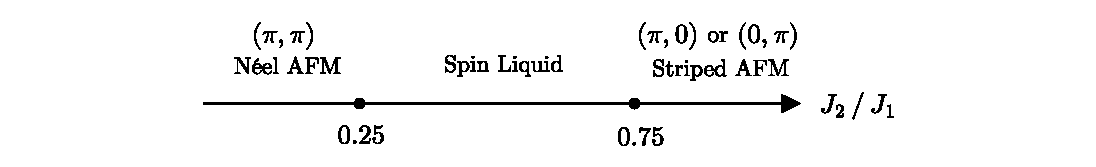
\includegraphics[width=\textwidth]{images/j1-j2/classical-expectation.pdf}
        \end{center}
    \end{subfigure}
    \caption{Ground State}
    \label{}
\end{figure}
%%% FIG %%%
% \FloatBarrier 
\!\!\!\!
Therefore, on comparing the energies, it is straightforward to see that the classical expectation of the phase boundaries at $T = 0$ is given as
\begin{align*}
    &0 \leq \frac{J_2}{J_1} \leq 0.25 \qquad \qquad \longrightarrow \text{ $(\pi, \pi)$ AFM} \\
    &0.25 \leq \frac{J_2}{J_1} \leq 0.75 \quad\qquad \longrightarrow \text{ Spin Liquid phase} \\
    &0.75 \leq \frac{J_2}{J_1} \qquad \qquad \qquad \longrightarrow \text{ $(\pi, 0)$ or $(0, \pi)$  AFM}
\end{align*}
Therefore, \textbf{exactly} at $T=0$, the phase transition in our effective model occurs at the points $J_2/J_1 = 0.25$ and $J_2/J_1 = 0.75$. However, as we'll discuss later, even a small temperature of $T\sim \mathcal{O}(\texttt{1.0e-1})$ can lead to the entropic stabilization of the AFM configurations and can play a huge role in shrinking the boundaries of the spin liquid phase to bring the semi-classically derived critical points closer to the quantum results.

\section{Semi-classical Monte Carlo} \label{SCMC}
Till now, we have proposed two important simplifications of the quantum $J_1-J_2$ Heisenberg model, i.e., 
\begin{enumerate}
    \item the quantum model is equivalent to a combination of $J_1-J_2$ Ising model and some effective quantum fluctuations.
    \item the quantum fluctuations can be modelled semi-classically by semi-classical dimers with zero magnetization and a temperature dependent energy $E(T)$ (Eq. \eqref{dimer}).
\end{enumerate}
To \textit{incorporate} the semi-classical dimers with the $J_1-J_2$ Ising model, we design a Metropolis Markov chain Monte Carlo algorithm with dimer creation and annihilation steps as Metropolis proposals. Roughly speaking, the Metropolis proposals consist of both spin flips and dimer creation-annihilation steps on the $J_1-J_2$ Ising lattice, and we expect the effects of the quantum fluctuations to revive in this semi-classical Monte Carlo simulation. A semi-classical Monte Carlo sweep is then defined as follows:
\begin{enumerate}
    \setlength\itemsep{0.1em}
    \item Randomly choose a site $i$ on the lattice.
    \item Check if the site $i$ is a part of the dimer or a free spin. 
    
    \item If site $i$ is a free spin, then we have two possible moves:
    \begin{itemize}[label={\textbf{--}}]
        \setlength{\itemsep}{0.1em}
        \item With a probability $p$, propose a spin flip $\sigma_i \to -\sigma_i$.
        \item With a probability $1-p$, propose the formation of a semi-classical dimer with another nearest or next-nearest neighbor free spin.
    \end{itemize}
    \item If the site $i$ is involved in a dimer (not a free spin), then propose the annihilation of the dimer and create two new random Ising spins. 
    \item Calculate the change in energy $\Delta E$. 
    \item Accept the proposed move with a probability of $\min \qty[e^{-\beta \Delta E}, 1]$.
    \item Steps $1$ to $6$ are then repeated $\mathcal{N} = L^2$ times.
\end{enumerate}
The probability $p$ is changed so as to tune the ratio of random spin-flip dynamics with dimer-formation dynamics. We will discuss the specifics of these parameters in the upcoming sections.

\section{Dimer dynamics in Monte Carlo} % Dimer creation and formation. MAKEFIGURE.
In this section, we will outline the idea behind the physics of creation and annihilation of dimers. The Monte Carlo dynamics is controlled by the change in energies. Hence, it is helpful to calculate the relevant expressions. 

Since the semi-classical dimer is a zero magnetization unit, it implies that the contribution of the neighbor interaction $S_i S_j = 0$ if $i$ or $j$ are part of a dimer. This can be encoded by \textbf{setting} $\boldsymbol{S_i = 0}$ \textbf{if site} $\boldsymbol{i}$ \textbf{is making a dimer with one of its neighbors}.
%%% FIG %%%
\begin{figure}[t!]
    \centering
    \begin{subfigure}[b]{0.8\textwidth}  %keep total sum <1 to show in same line
        \centering
        \includegraphics[width=\textwidth]{images/j1-j2/dimer.tex}
    \end{subfigure}
    \caption{Semi-classical dimer formation on $\expval{i, j}$  with $S_i = S_j = 0$ and $E = E_J(T)$.}
    \label{}
\end{figure}
%%% FIG %%%
\FloatBarrier \!\!\!\!\!\!\!\!\!\!\!
On the basis of this setup, we can calculate the changes in energy in a dimer creation or annihilation process. Let's say a dimer is created between sites $i = (i_x, i_y)$ and $j = (j_x, j_y)$. The change in energy due to dimer creation is then given by
\begin{align*}
    \Delta E_\text{c} =  & + E_J(T) -\frac{J_1}{4} \qty[S_{(i_x, i_y)} \!\!\!\!\!\!\!\! \sum_{\vec{\delta} \in \{(0,\pm 1), (\pm 1, 0) \}} \!\!\!\!\!\!\!\! S_{(i_x, i_y) + \vec{\delta}} \quad + S_{(j_x, j_y)} \!\!\!\!\!\!\!\! \sum_{\vec{\delta} \in \{(0,\pm 1), (\pm 1, 0) \}} \!\!\!\!\!\!\!\! S_{(j_x, j_y) + \vec{\delta}}] \\
    & -\frac{J_2}{4} \qty[S_{(i_x, i_y)} \!\!\!\!\!\!\!\! \sum_{\vec{\delta} \in \{(1,\pm 1), (-1,\pm 1) \}} \!\!\!\!\!\!\!\! S_{(i_x, i_y) + \vec{\delta}} \quad + S_{(j_x, j_y)} \!\!\!\!\!\!\!\! \sum_{\vec{\delta} \in \{(1,\pm 1), (-1,\pm 1) \}} \!\!\!\!\!\!\!\! S_{(j_x, j_y) + \vec{\delta}}] + \frac{J}{4} S_{(i_x, i_y)} S_{(j_x, j_y)}
\end{align*}
where $J$ is equal to $J_1$ or $J_2$ depending on whether the dimer is formed with the nearest or next-nearest neighbor, respectively, and the Ising spin configuration $\{S_{(x,y)}\}$ is the set of values before the dimer is formed.

Similarly, the change in energy due to annihilation of the dimer between sites $i$ and $j$ and creation of two free spins is given by
\begin{align*}
    \Delta E_\text{a} =  & -E_J(T) +\frac{J_1}{4} \qty[S'_{(i_x, i_y)} \!\!\!\!\!\!\!\! \sum_{\vec{\delta} \in \{(0,\pm 1), (\pm 1, 0) \}} \!\!\!\!\!\!\!\! S'_{(i_x, i_y) + \vec{\delta}} \quad + S'_{(j_x, j_y)} \!\!\!\!\!\!\!\! \sum_{\vec{\delta} \in \{(0,\pm 1), (\pm 1, 0) \}} \!\!\!\!\!\!\!\! S'_{(j_x, j_y) + \vec{\delta}}] \\
    & +\frac{J_2}{4} \qty[S'_{(i_x, i_y)} \!\!\!\!\!\!\!\! \sum_{\vec{\delta} \in \{(1,\pm 1), (-1,\pm 1) \}} \!\!\!\!\!\!\!\! S'_{(i_x, i_y) + \vec{\delta}} \quad + S'_{(j_x, j_y)} \!\!\!\!\!\!\!\! \sum_{\vec{\delta} \in \{(1,\pm 1), (-1,\pm 1) \}} \!\!\!\!\!\!\!\! S'_{(j_x, j_y) + \vec{\delta}}] - \frac{J}{4} S'_{(i_x, i_y)} S'_{(j_x, j_y)}
\end{align*}
where again $J$ is equal to $J_1$ or $J_2$ depending on whether it was a nearest or next-nearest neighbor dimer, respectively, and the spin configuration $\{S'_{(x,y)}\}$ is the set of values after the two new random spins are formed in place of the dimer.
\section{Simulations and results}
Now that we have our machinery ready, we implement the Metropolis Monte Carlo algorithm as discussed in Sec. \ref{SCMC} with a combination of spin flips and dimer creation/annihilation steps.

We use the following simulation parameters for the semi-classical Monte Carlo simulations of the $J_1-J_2$ Heisenberg model.
\begin{itemize}[label={}] 
    \setlength{\itemsep}{0.1em}   
    \item \texttt{lattice size = 10 $\cross$ 10}
    \item \texttt{J${}_1$ = 4.0}
    \item \texttt{J${}_2/\texttt{J}_1 \in [\texttt{0.1}, \texttt{0.2}, \ldots, \texttt{1.0}]$ }
    \item \texttt{T} $\in [\texttt{0.1}, \texttt{0.2}, \ldots, \texttt{4.0}]$ \texttt{(with thermal annealing)}
    \item \texttt{no of equilibration sweeps = 1.0e3}
    \item \texttt{no of sampling sweeps = 5.0e3}
\end{itemize}
From preliminary studies, we are aware that the $J_1 - J_2$ Heisenberg model exhibits four different quantum phases $-$ the $(\pi, \pi)$ AFM, the spin liquid (quantum paramagnet state), the $(\pi, 0)$ or $(0, \pi)$ AFM, or the thermal paramagnetic phase. Therefore, we require $4 - 1 = 3$ different order parameters to characterize these phases. We define the following three order parameters.
\begin{itemize}
    \setlength{\itemsep}{0.1em}   
    \item Staggered magnetizaton $(\pi, \pi)$ 
    \[ 
        m_{(\pi, \pi)} = \frac{1}{L^2} \sum_{i = 1}^{L^2} (-1)^{i_{x} + i_{y}}\: S_i
    \]
    \item Staggered magnetizaton $(\pi, 0)$ and $(0, \pi)$  
    \[ 
        m_{(\pi, 0)} +  m_{(0, \pi)} = \frac{1}{L^2} \sum_{i = 1}^{L^2} \qty[(-1)^{i_{x}} + (-1)^{i_{y}}] \: S_i 
    \]
    \item Number of dimers
    \[
        N_\text{dimers} = N_{J_1 \text{ dimers}} + N_{J_2 \text{ dimers}}
    \]
\end{itemize}
Further, we also have the parameter $p$, which is defined as the ratio of random spin flips to dimer creation steps, which we haven't fixed yet. Since $p$ is a parameter which doesn't explicitly depend upon the model but is an artefact of the design of the algorithm, one needs a way to define what a ``good'' value of $p$ is. We'll defer this problem to the next section and explore the phase diagrams with different values of $p$ for now.
\subsection{Phase Diagrams}
As can be seen from the phase diagrams, we have all the expected phases emerging from the semi-classical Monte Carlo calculation which are also found from an exact quantum calculation. As a very first step, this shows that it is indeed possible for \textbf{quantum phases to emerge by adding quantum fluctuations on top of a classical model.} In fact, the qualitative features of the phase diagram obtained using our semi-classical Monte Carlo approach matches with the essential features of the phase diagram obtained through a cluster mean-field theory calculation of the $J_1-J_2$ Heisenberg model, as shown in Fig. \ref{CMFT}. 

%%% FIG %%%
\begin{figure}[!htb]
    \centering
    \begin{subfigure}[b]{0.6\textwidth}  %keep total sum <1 to show in same line
        \centering
        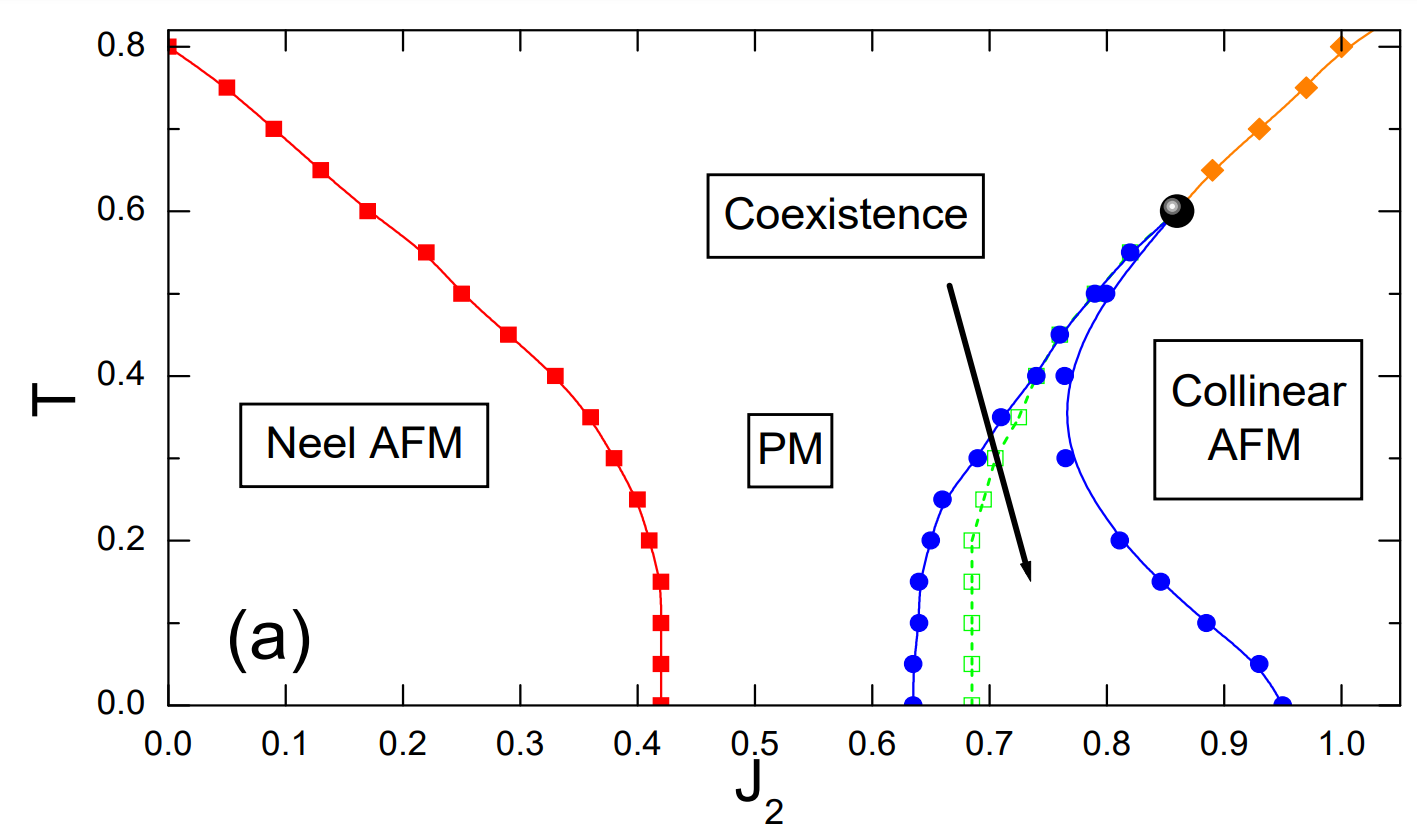
\includegraphics[width=\textwidth]{images/j1-j2/CMFT_diagram.png}
    \end{subfigure}
    \caption{Phase diagram of $J_{1}$-$J_{2}$ model in the $T-J_{2}$ plane, obtained
    using $2 \times 2$ cluster mean-field theory. Squares with eye
    guiding line is the second-order N$\acute{e}$el-to-paramagnetic phase transition.
    Solid dots represent coexistence boundaries of paramagnetic phase and
    collinear AFM phase. The empty squares with dashed line is the actual transition line
    of equal free energy. The solid dot at ($J_{2c}=0.86$, $T_{c}=0.6$) is the critical point above which the
  first-order transition changes into a second-order line (diamonds
  with solid line) \cite{Ren_2014}.}
    \label{CMFT}
\end{figure}
%%% FIG %%%
\FloatBarrier \!\!\!\!\!\!\!\!\!\!\!
However, as one can notice, the phase boundaries of the Néel AFM to spin liquid, and the spin liquid to the collinear/striped AFM phase transitions does not exactly match with the standard values of $J_2/J_1 \sim 0.4$ and $J_2/J_1 \sim 0.6$, respectively. In fact, the quantum critical points as found from a semi-classical Monte Carlo simulation depends upon the parameter $p$ (and not on the number of sampling sweeps, as expected). The Figures \ref{p=0.15}, \ref{p=0.25}, and \ref{p=0.50} clearly an increase in the width of the phase boundaries of the spin liquid phase as the value of $p$ is increased. A possible explanation may underline the fact that an increase in the value of $p$ increases the probability of dimer formation which ends up creating a meta-stable fully dimerized state even in the regimes where it is not fully stable. However, as a working definition ``correct'' value of $p$ can be chosen as the parameter value which maximizes the acceptance rate of the Monte Carlo algorithm.
%%% FIG %%%
\begin{figure}[!htb]
    \centering
    \begin{subfigure}[b]{0.43\textwidth}  %keep total sum <1 to show in same line
        \centering
        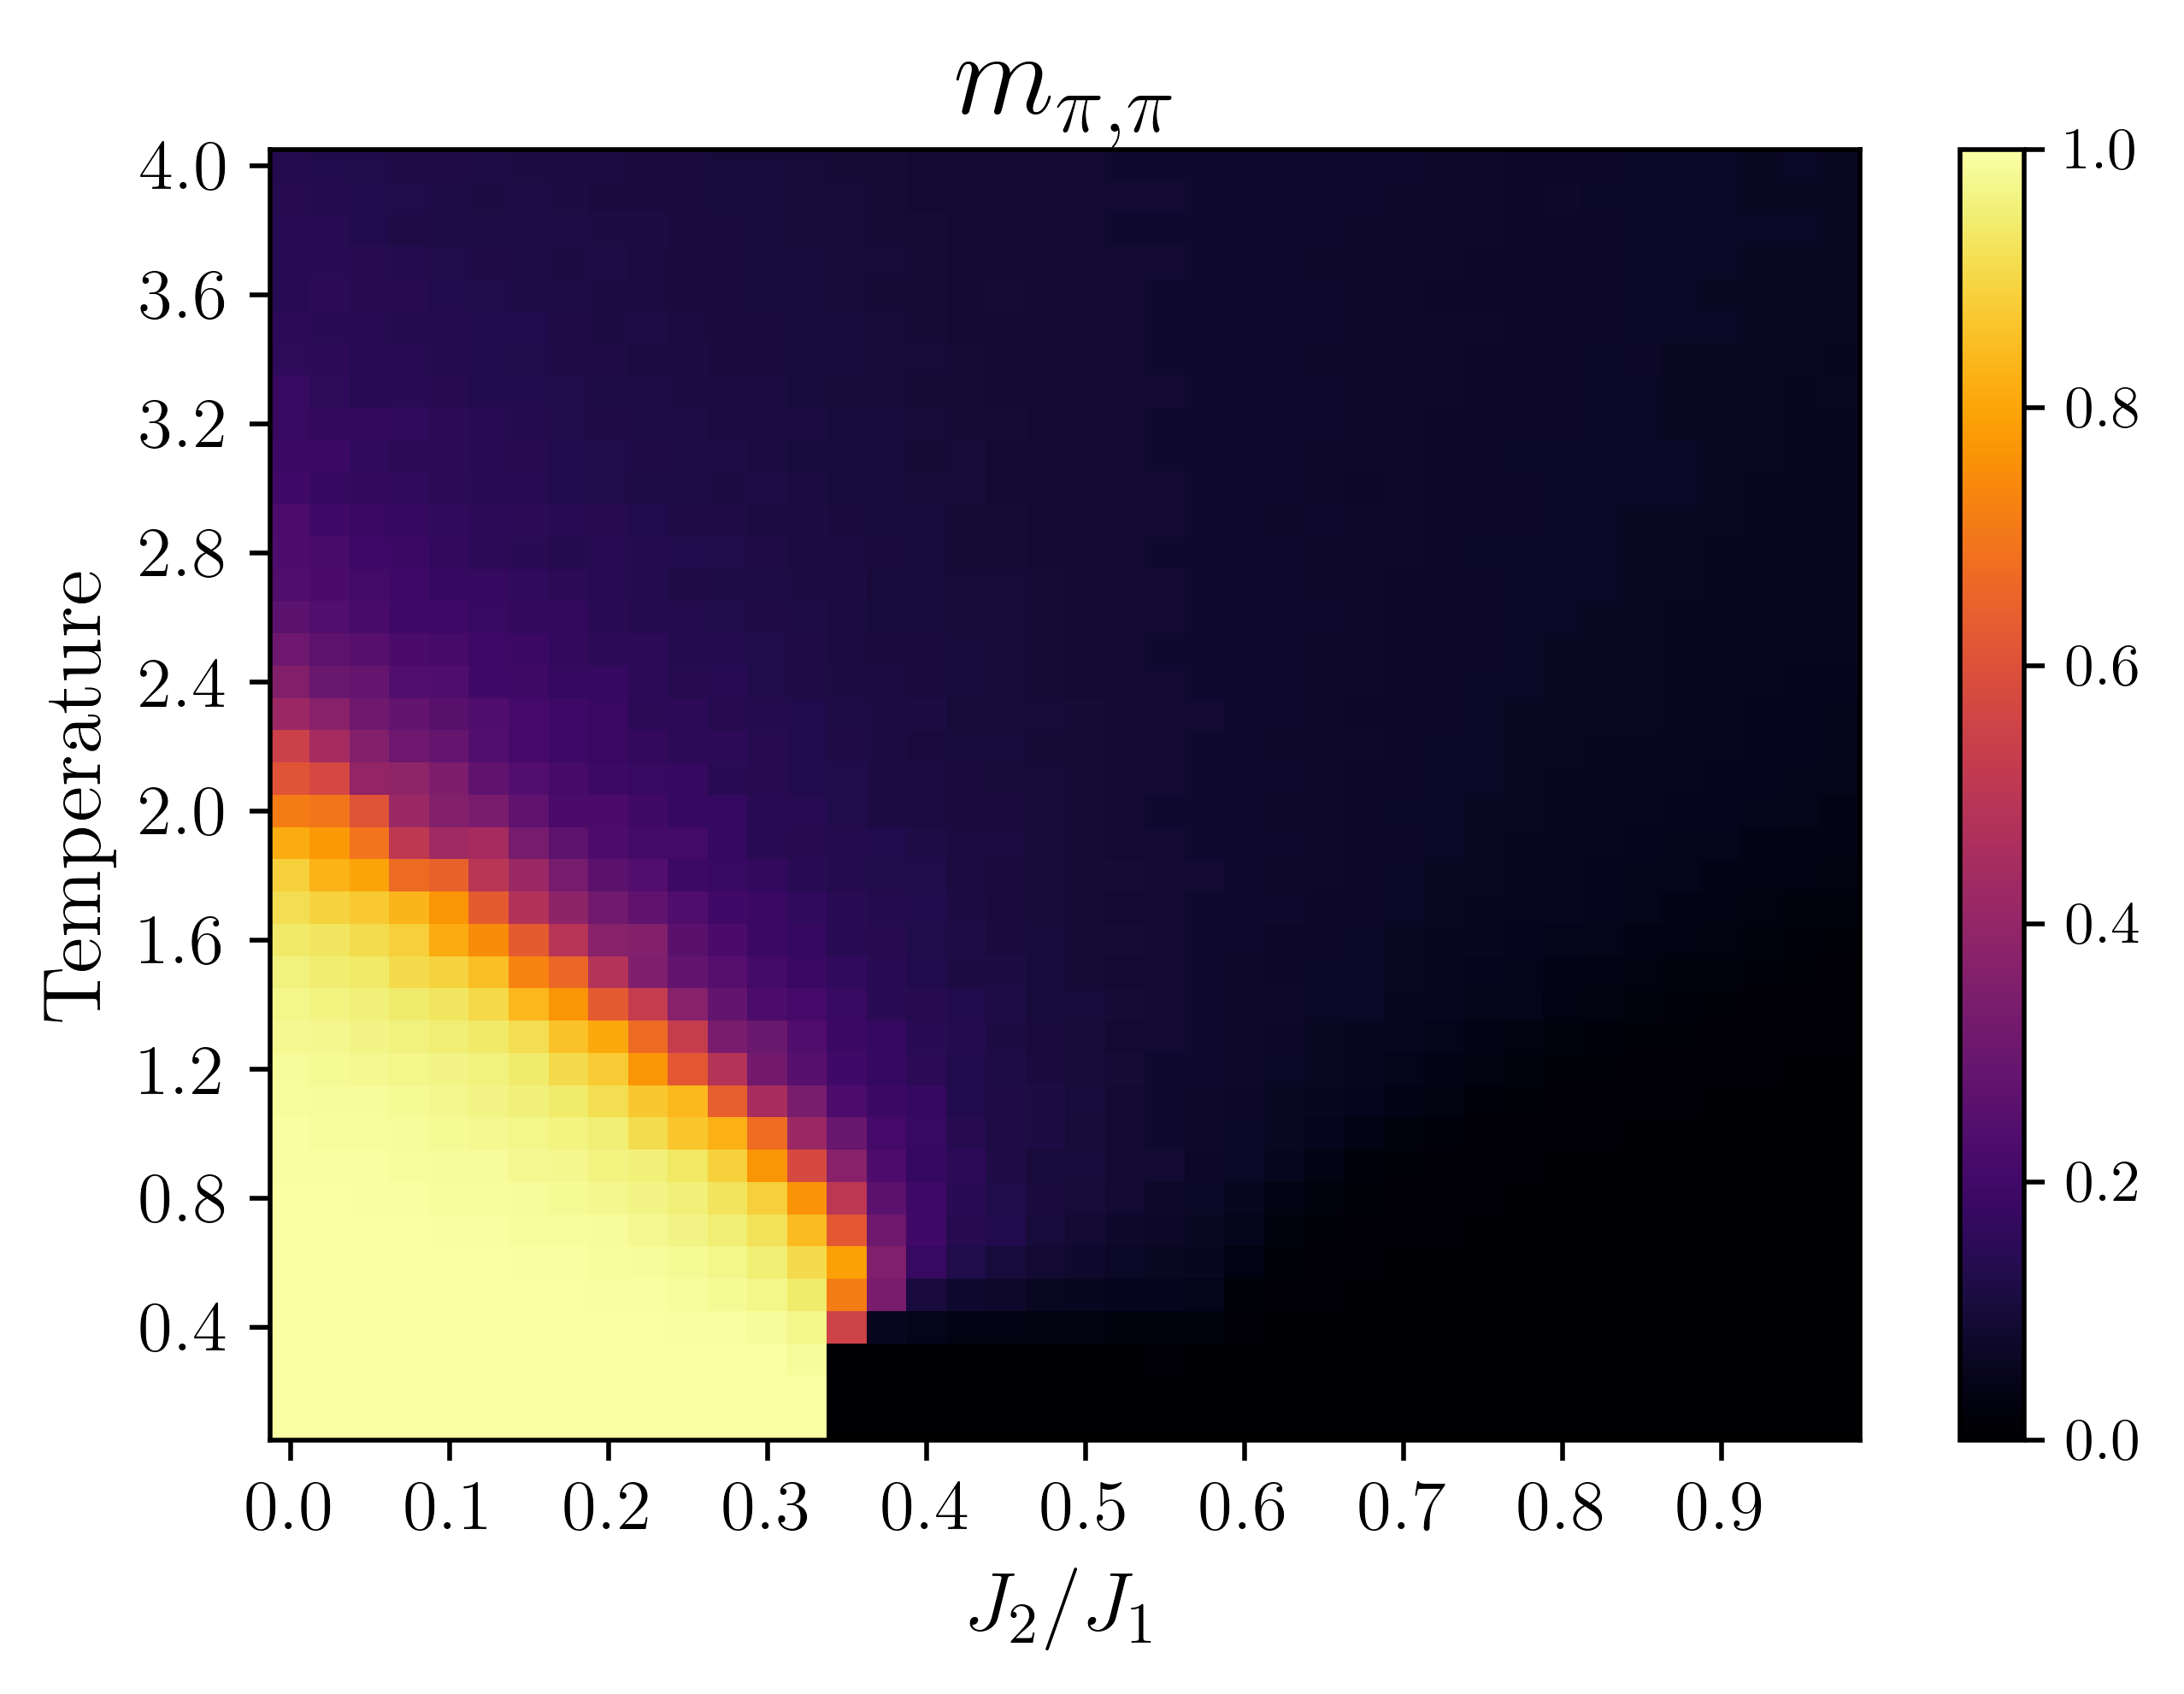
\includegraphics[width=\textwidth]{images/j1-j2/phase_diagrams/p=0.15/M_pi,pi_p=0.15.png}
    \end{subfigure}
    \begin{subfigure}[b]{0.43\textwidth}
        \centering
        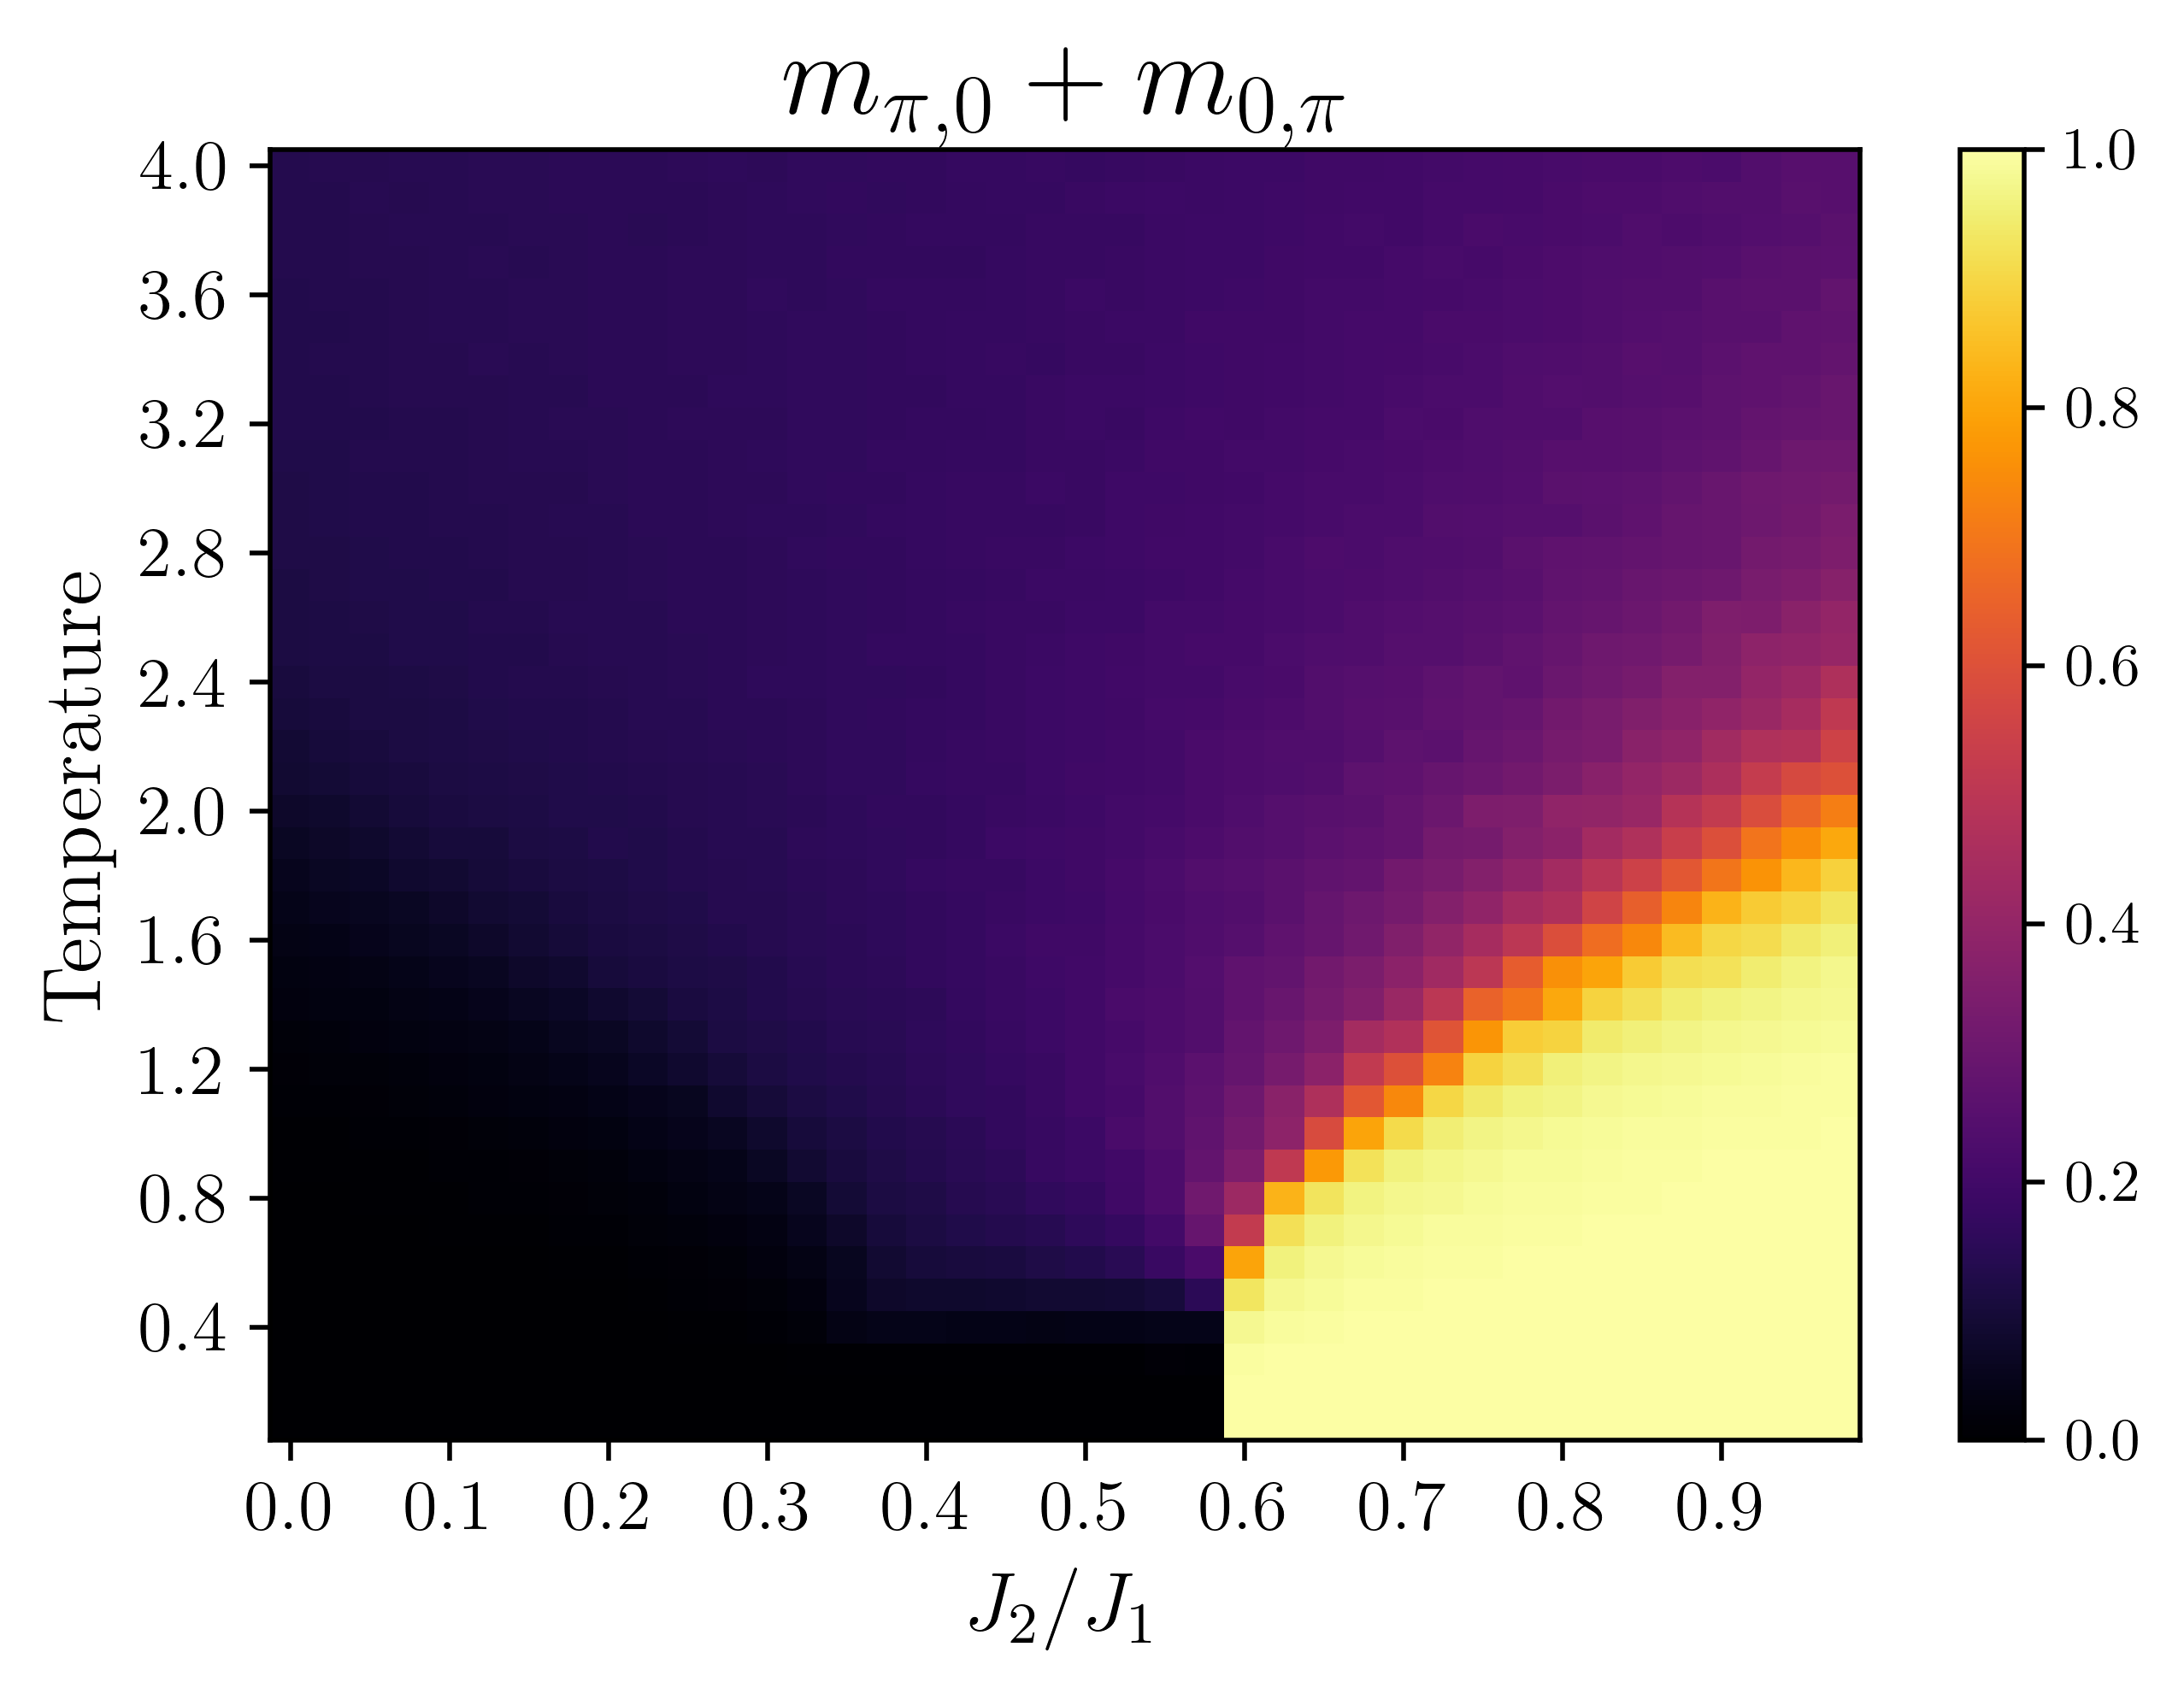
\includegraphics[width=\textwidth]{images/j1-j2/phase_diagrams/p=0.15/M_pi,0_p=0.15.png}
    \end{subfigure}
    \begin{subfigure}[b]{0.43\textwidth}
        \centering
        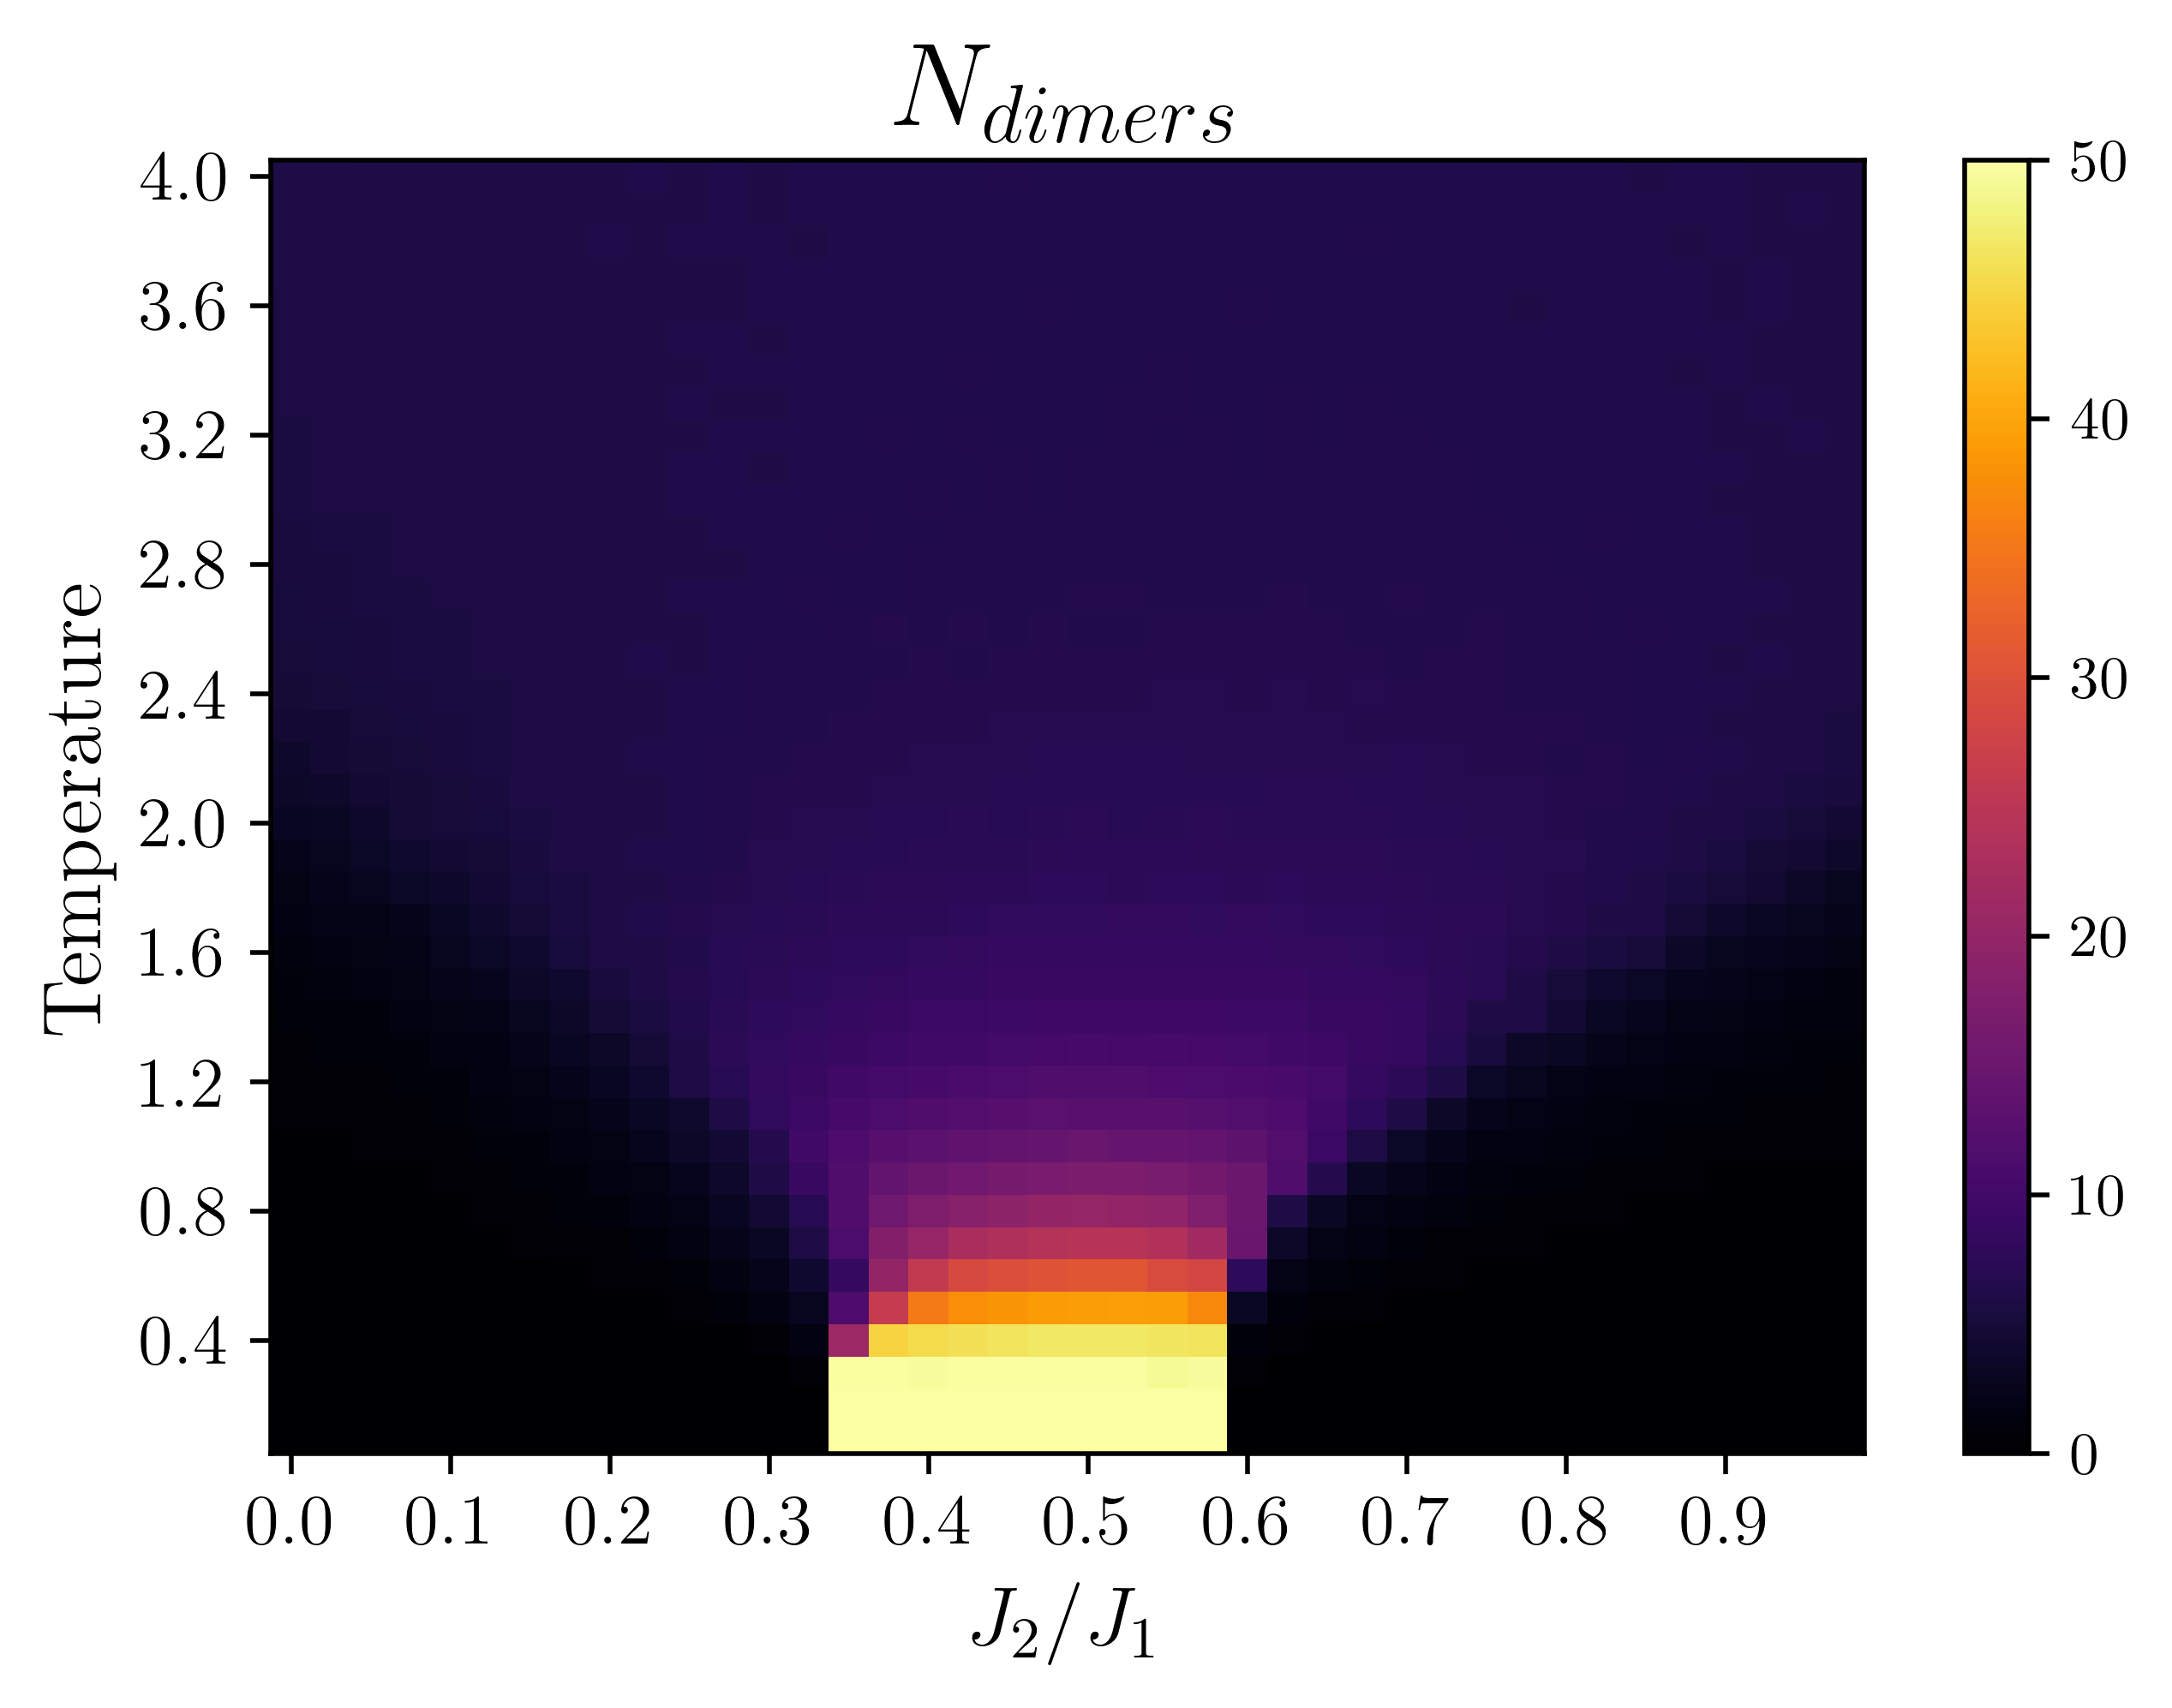
\includegraphics[width=\textwidth]{images/j1-j2/phase_diagrams/p=0.15/N_dimers_p=0.15.png}
    \end{subfigure}
    \caption{Order parameters at $p = 0.15$}
    \label{p=0.15}
\end{figure}
%%% FIG %%%
\FloatBarrier
%%% FIG %%%
\begin{figure}[!htb]
    \centering
    \begin{subfigure}[b]{0.43\textwidth}  %keep total sum <1 to show in same line
        \centering
        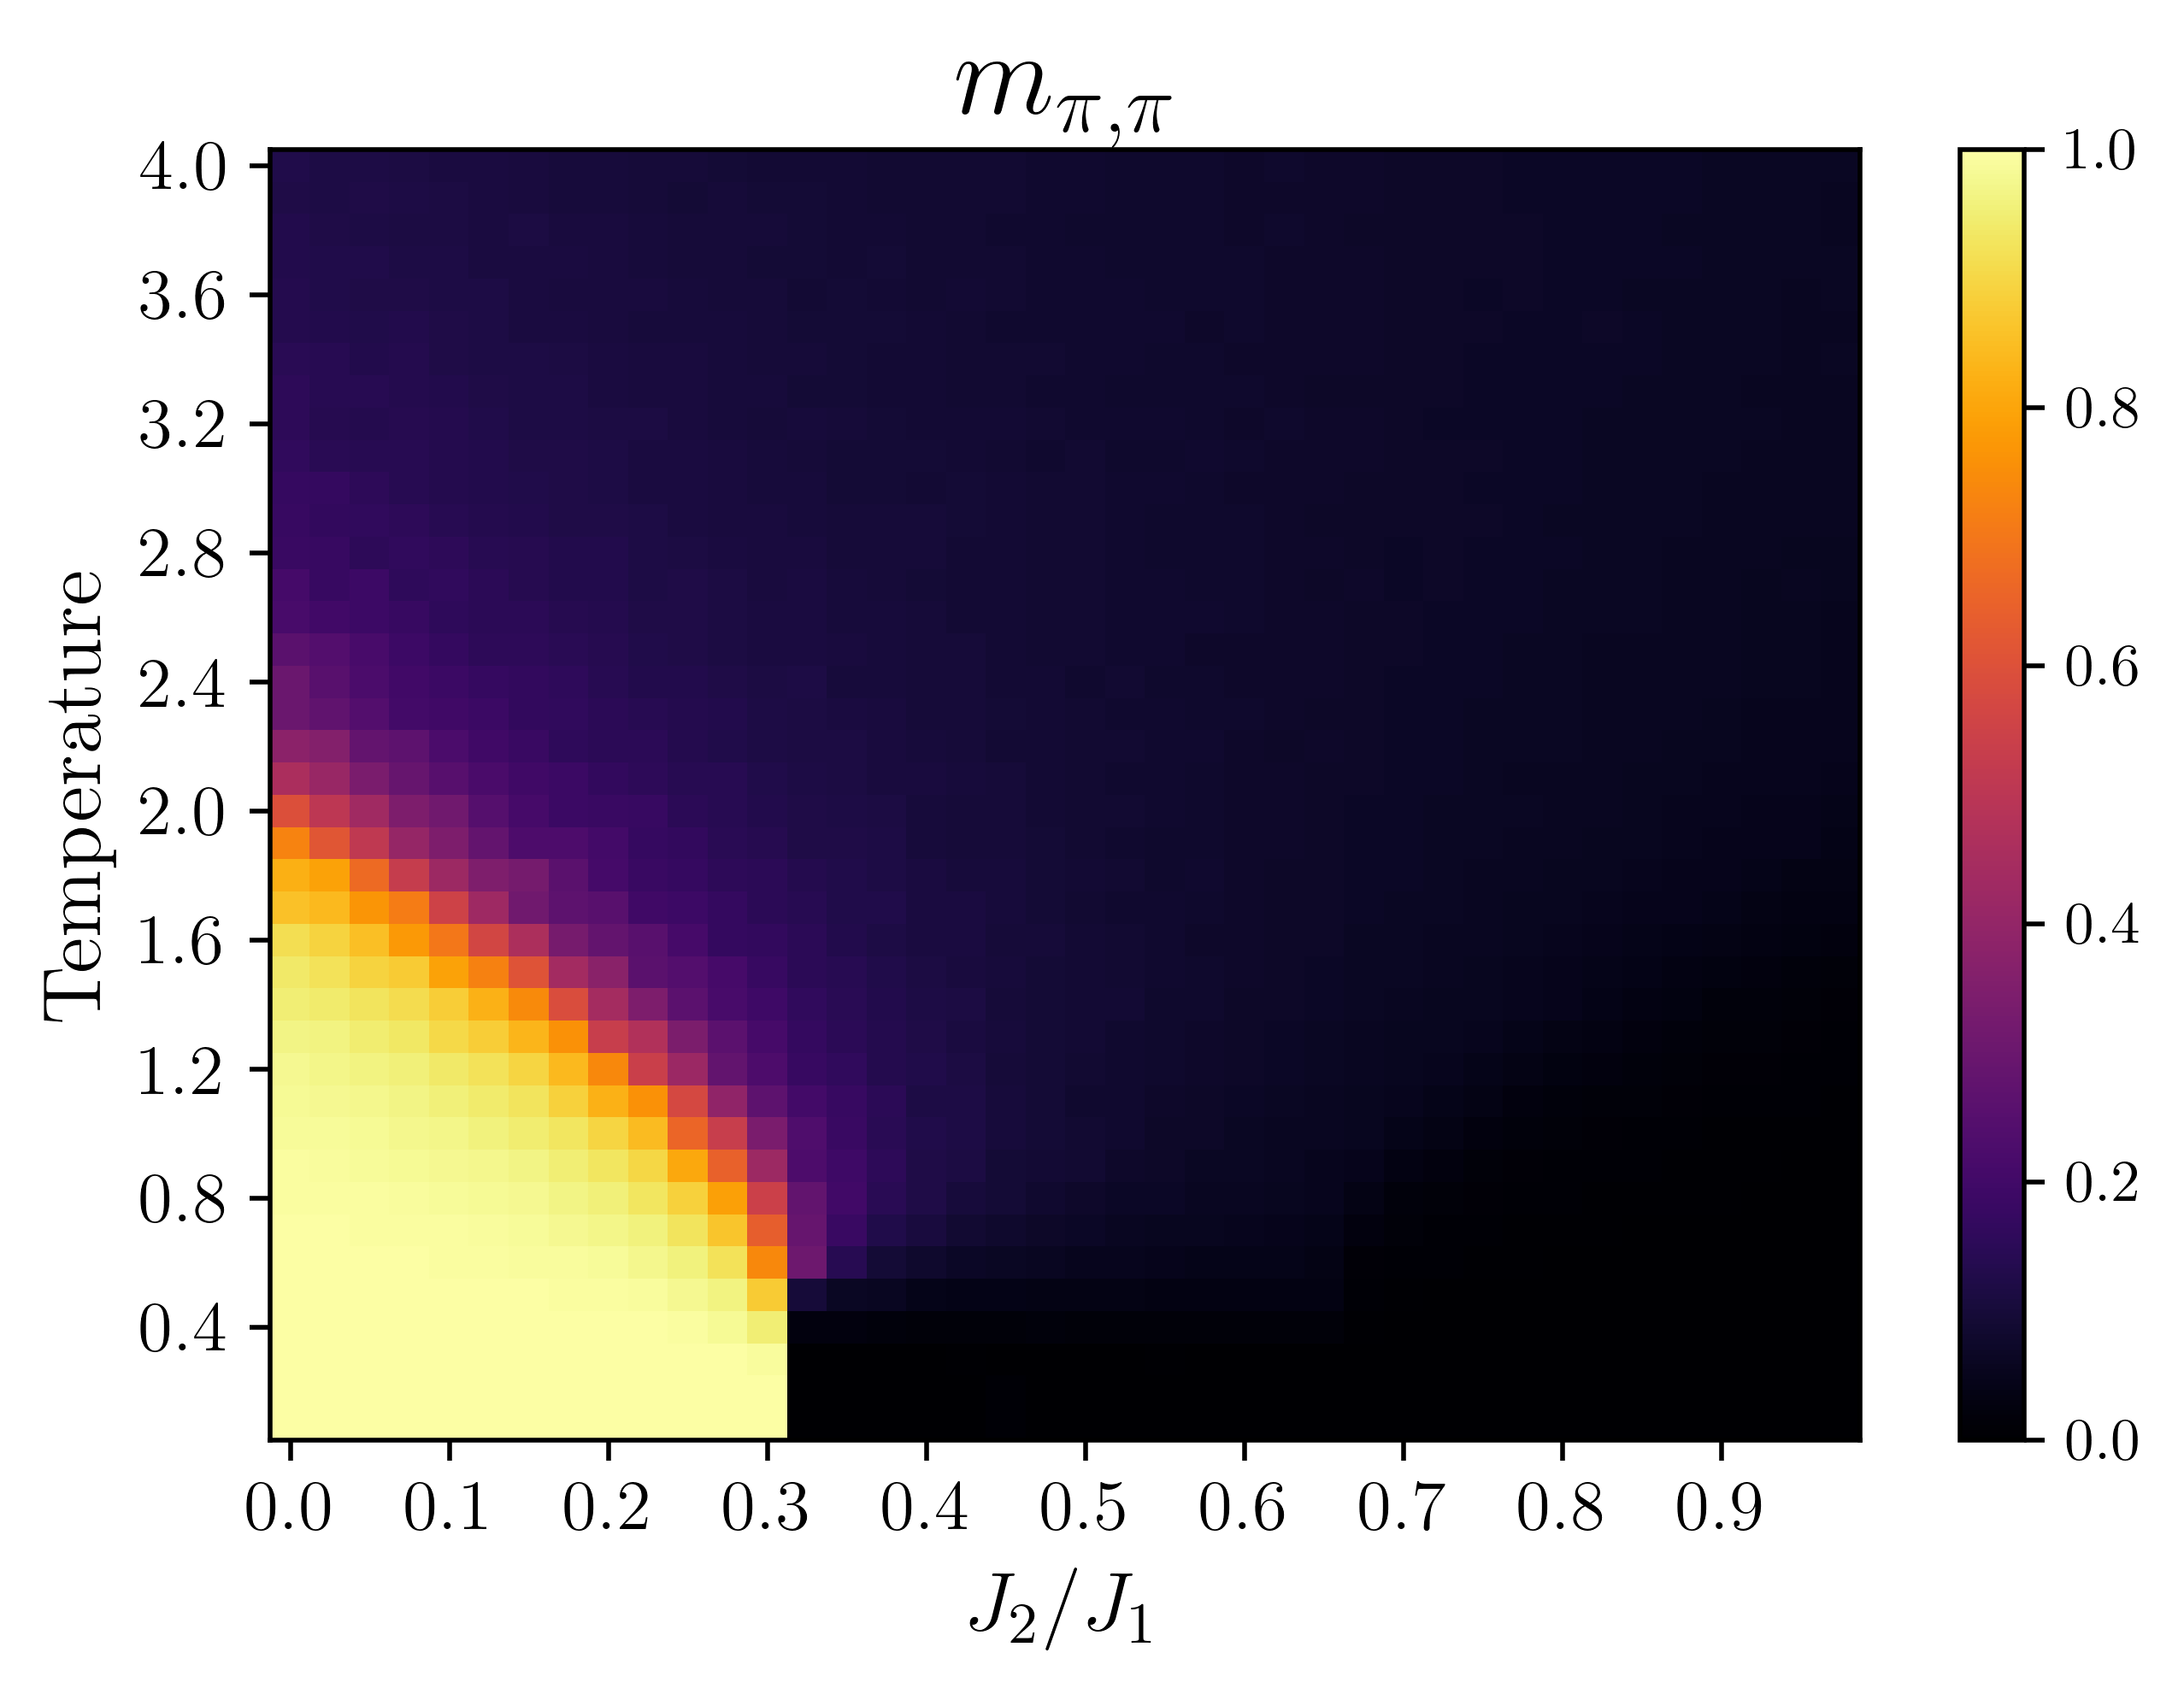
\includegraphics[width=\textwidth]{images/j1-j2/phase_diagrams/p=0.25/M_pi,pi_p=0.25.png}
    \end{subfigure}
    \begin{subfigure}[b]{0.43\textwidth}
        \centering
        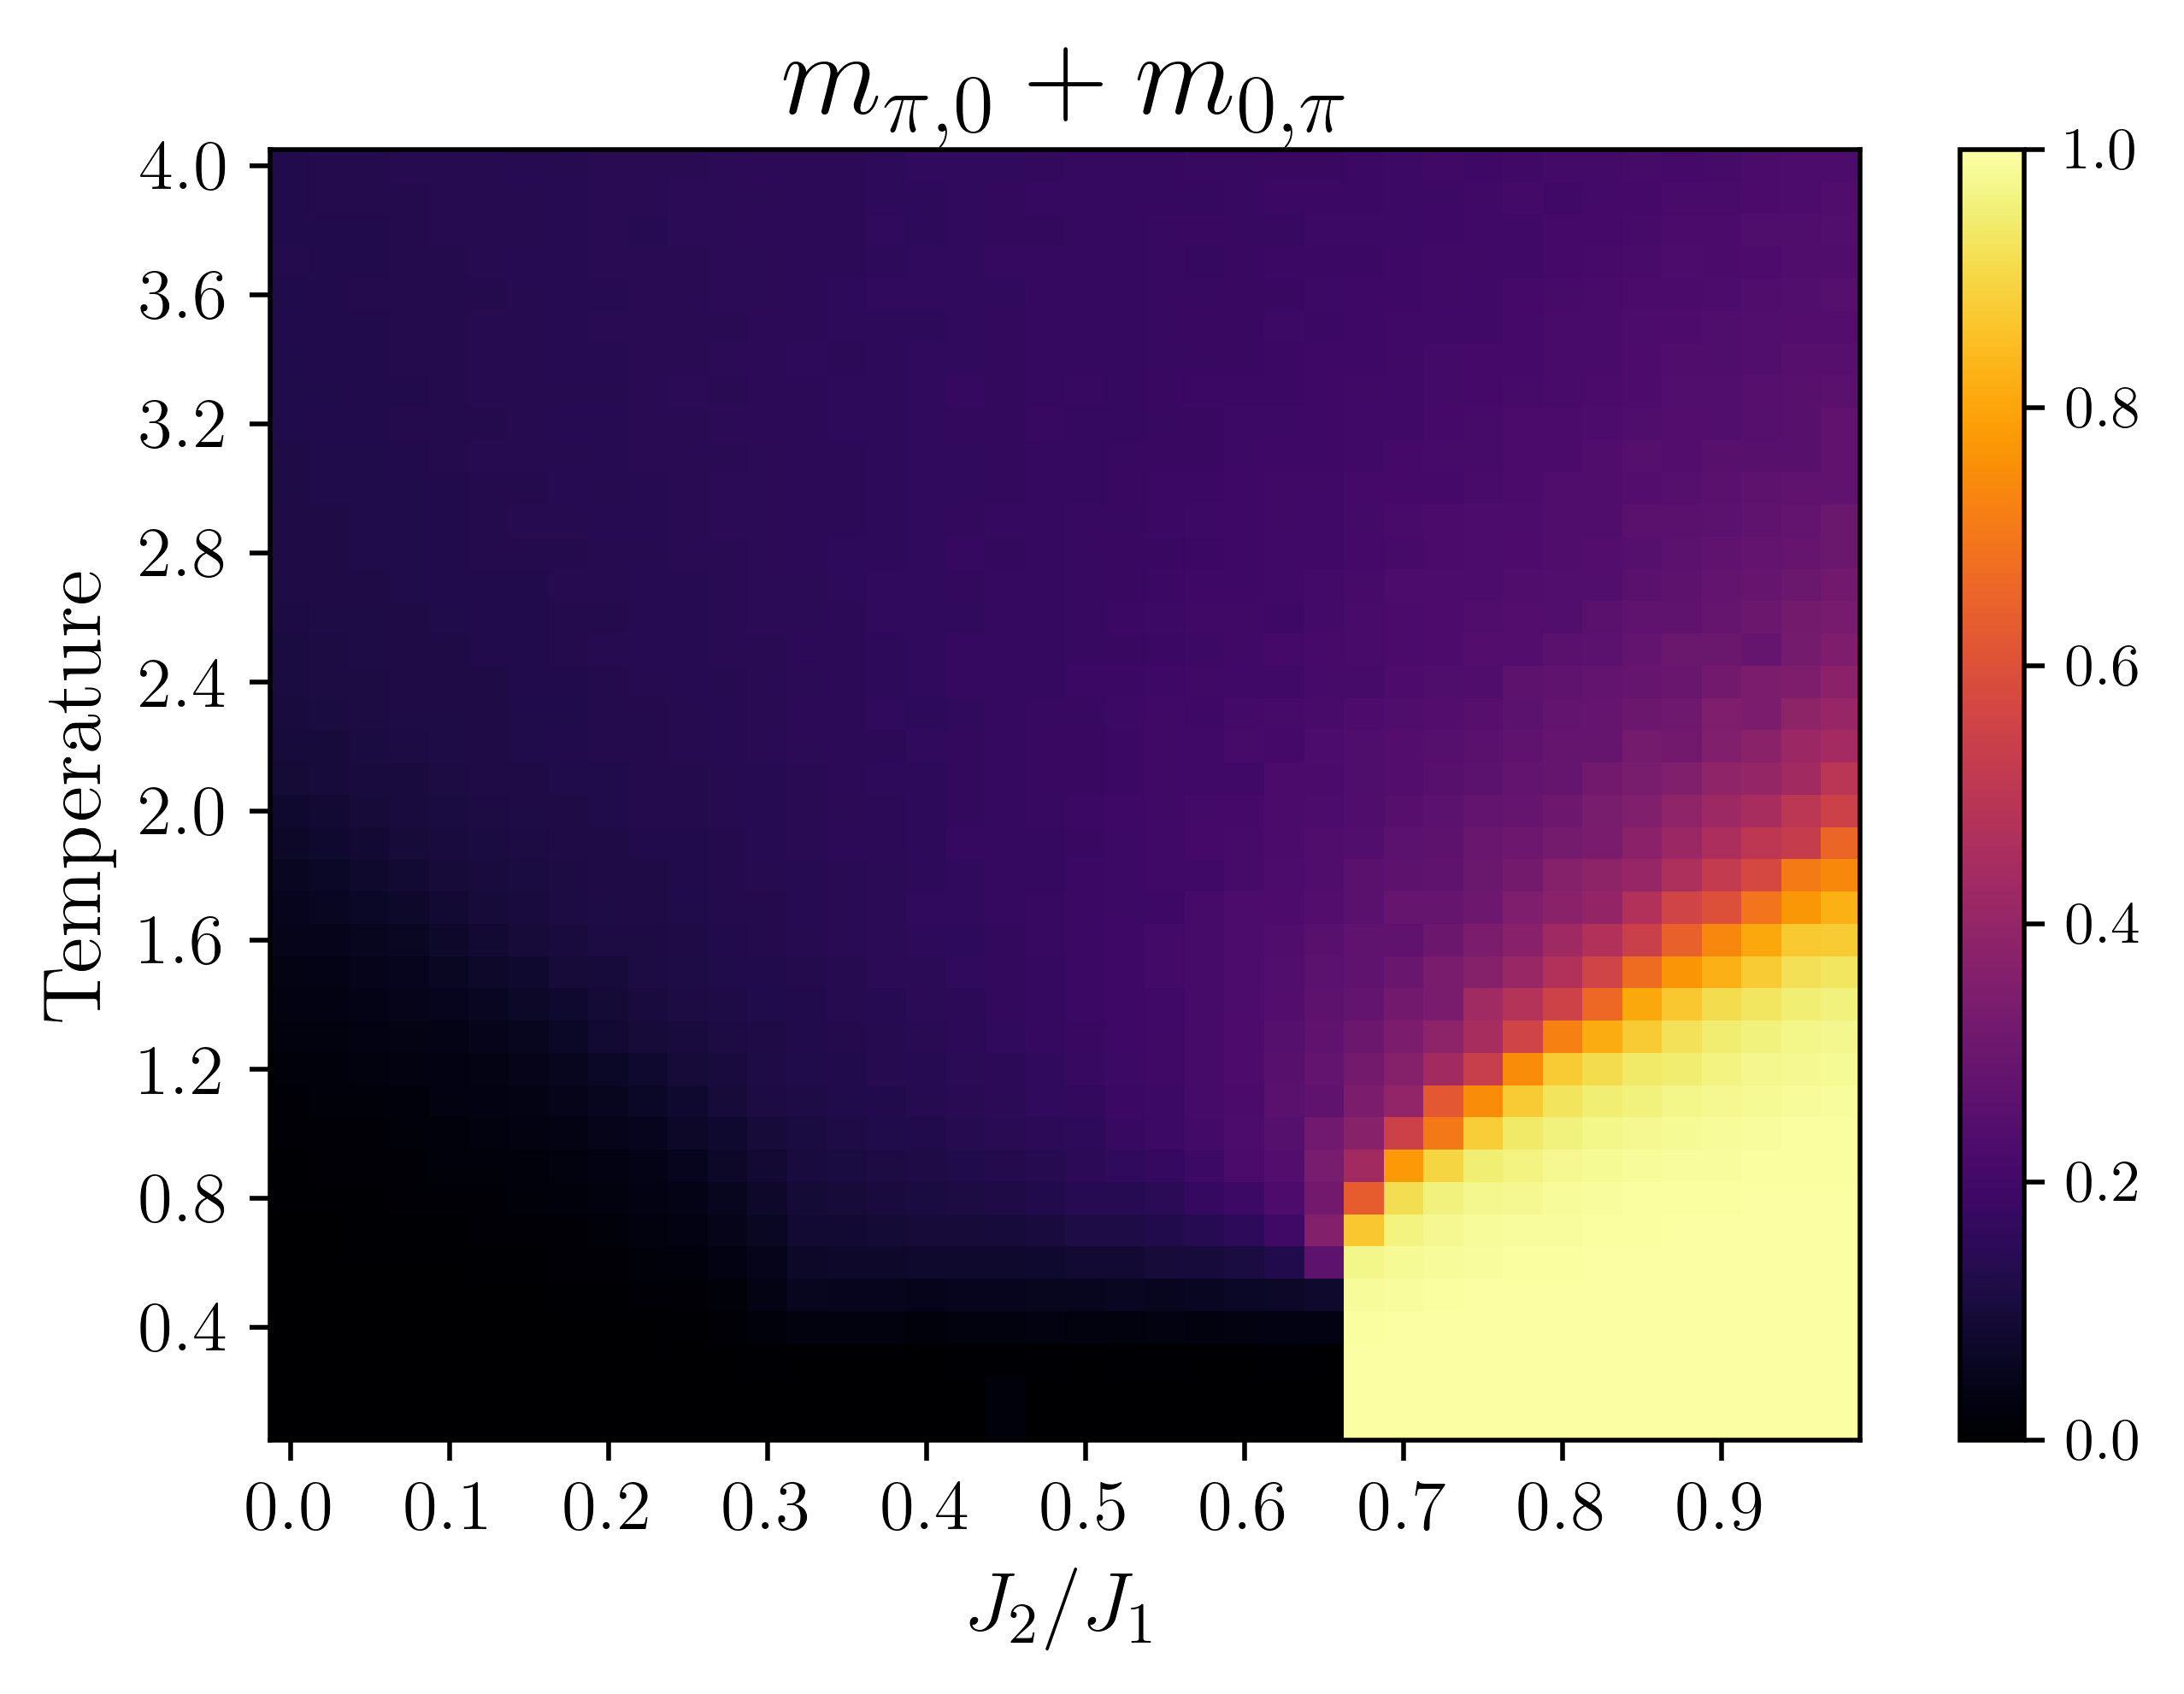
\includegraphics[width=\textwidth]{images/j1-j2/phase_diagrams/p=0.25/M_pi,0_p=0.25.png}
    \end{subfigure}
    \begin{subfigure}[b]{0.43\textwidth}
        \centering
        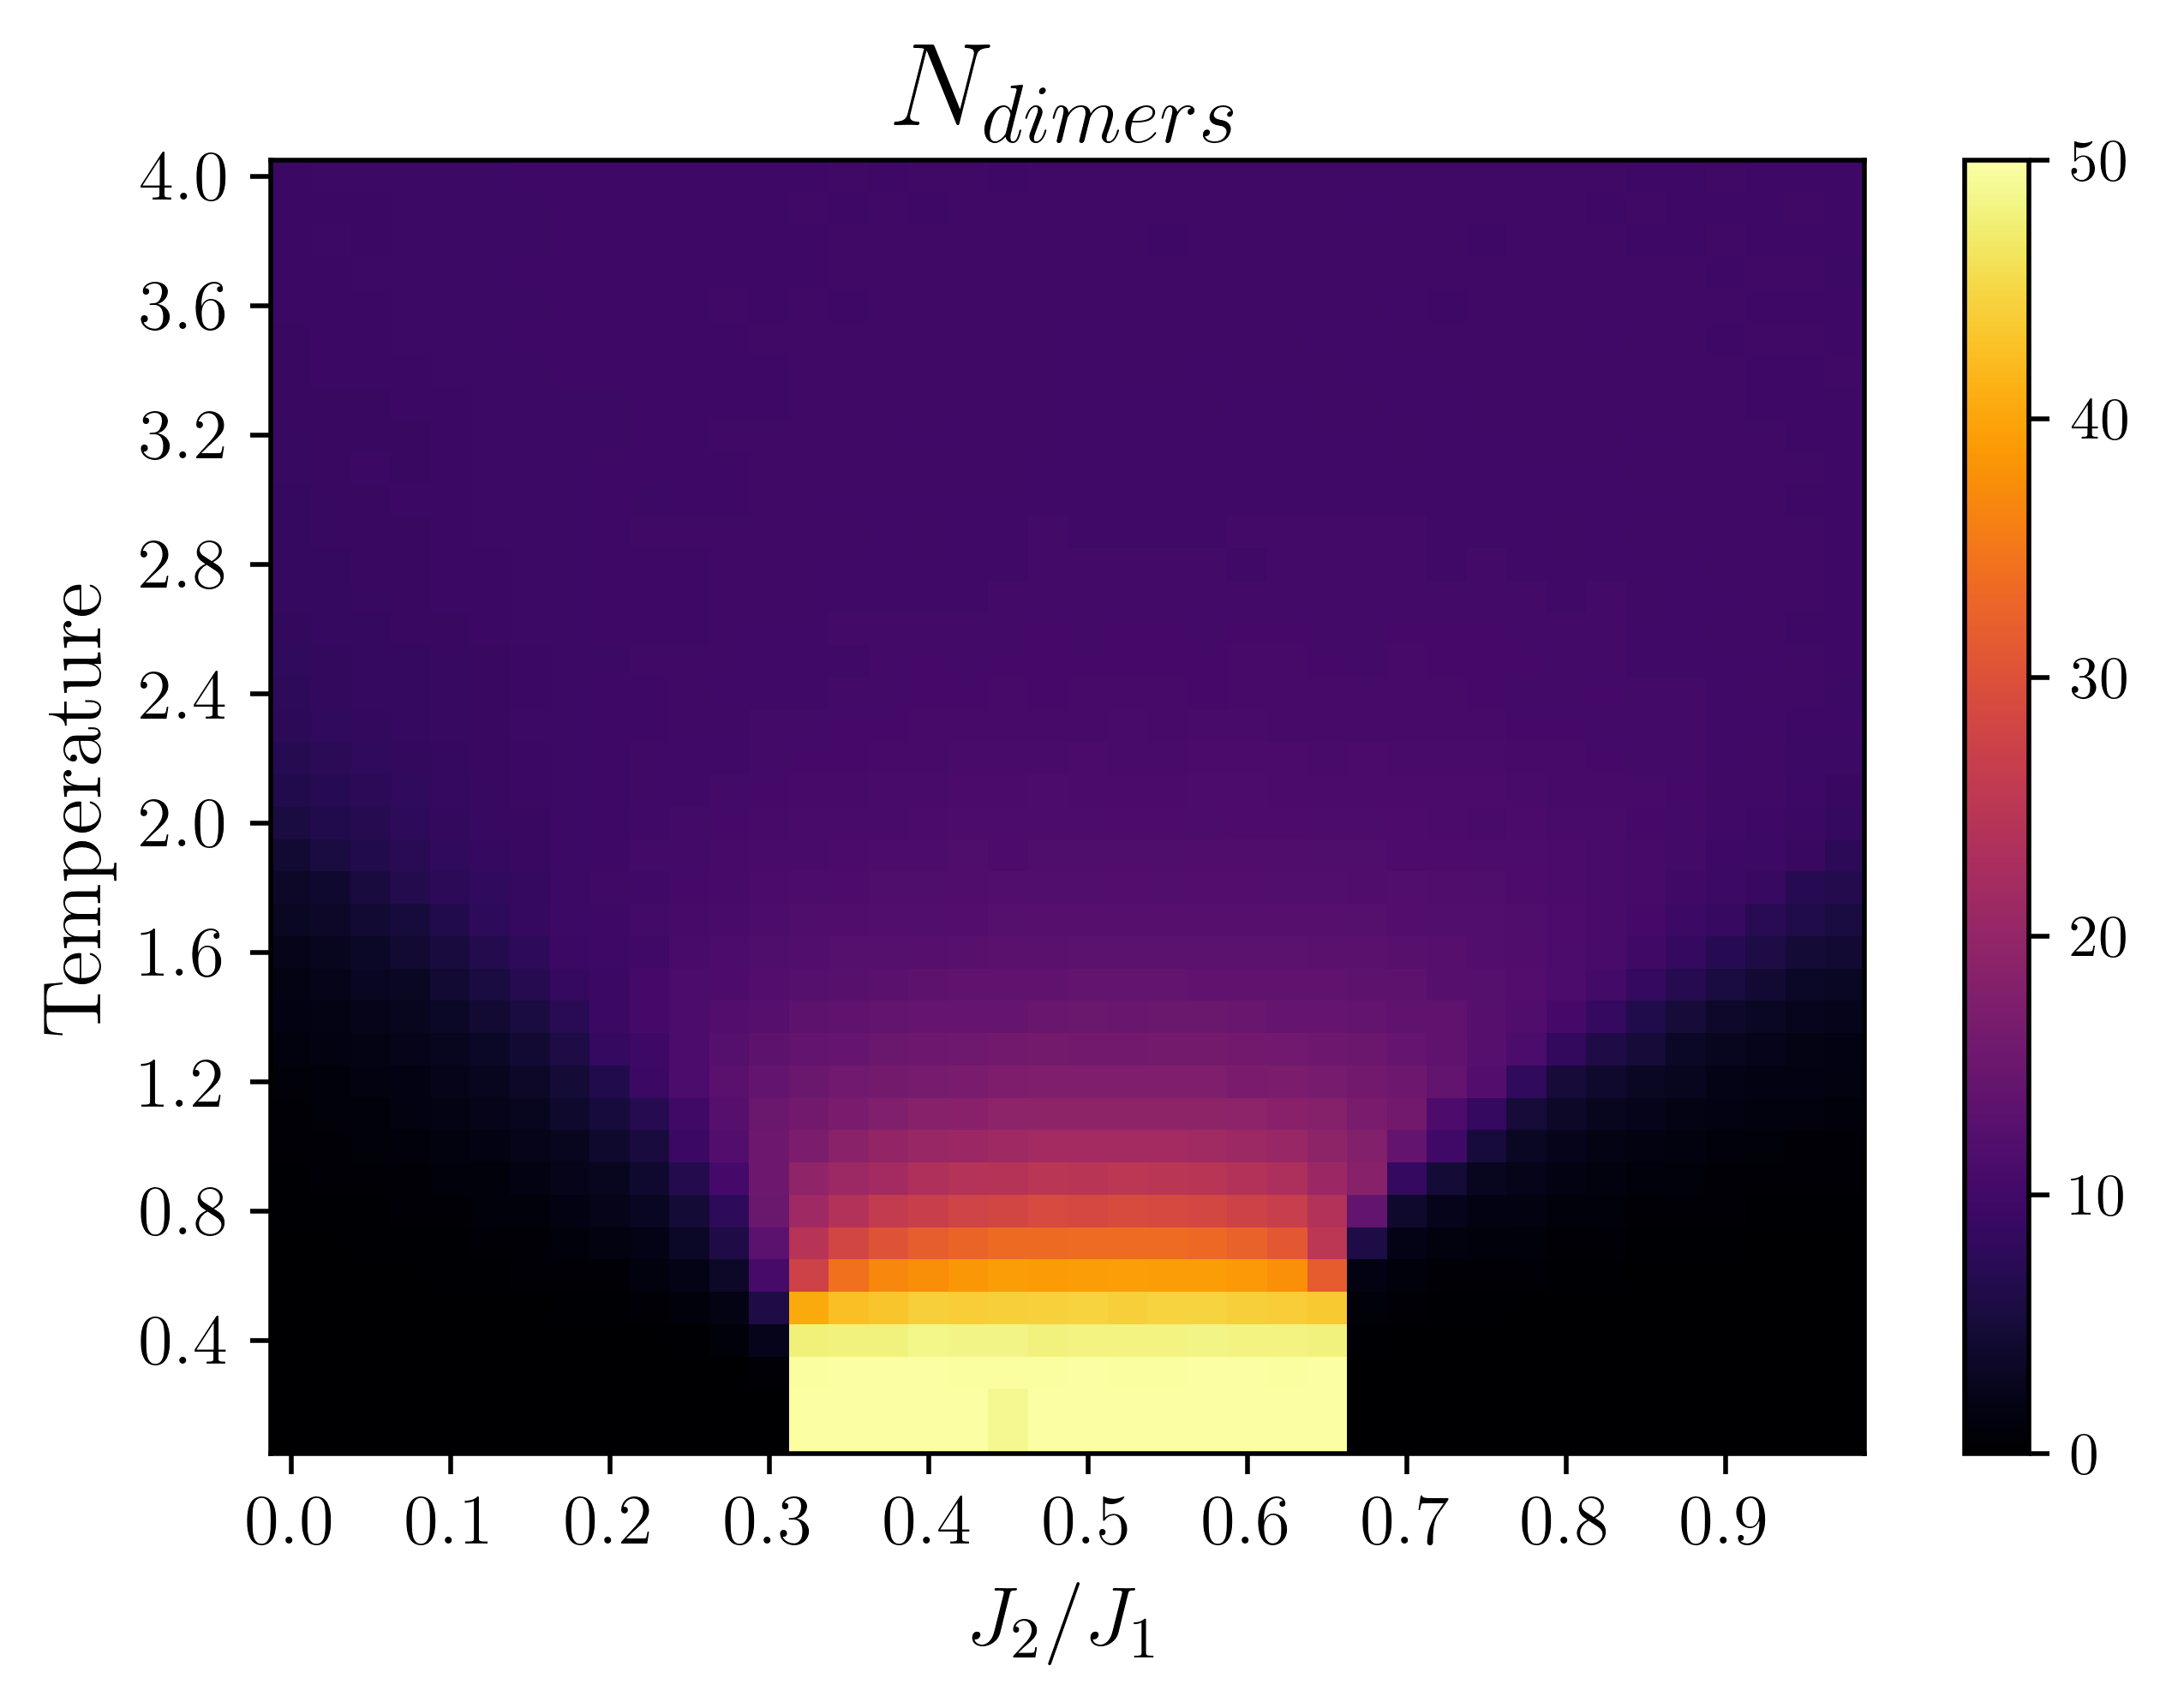
\includegraphics[width=\textwidth]{images/j1-j2/phase_diagrams/p=0.25/N_dimers_p=0.25.png}
    \end{subfigure}
    \caption{Order parameters at $p = 0.25$}
    \label{p=0.25}
\end{figure}
%%% FIG %%%
\FloatBarrier
%%% FIG %%%
\begin{figure}[!htb]
    \centering
    \begin{subfigure}[b]{0.43\textwidth}  %keep total sum <1 to show in same line
        \centering
        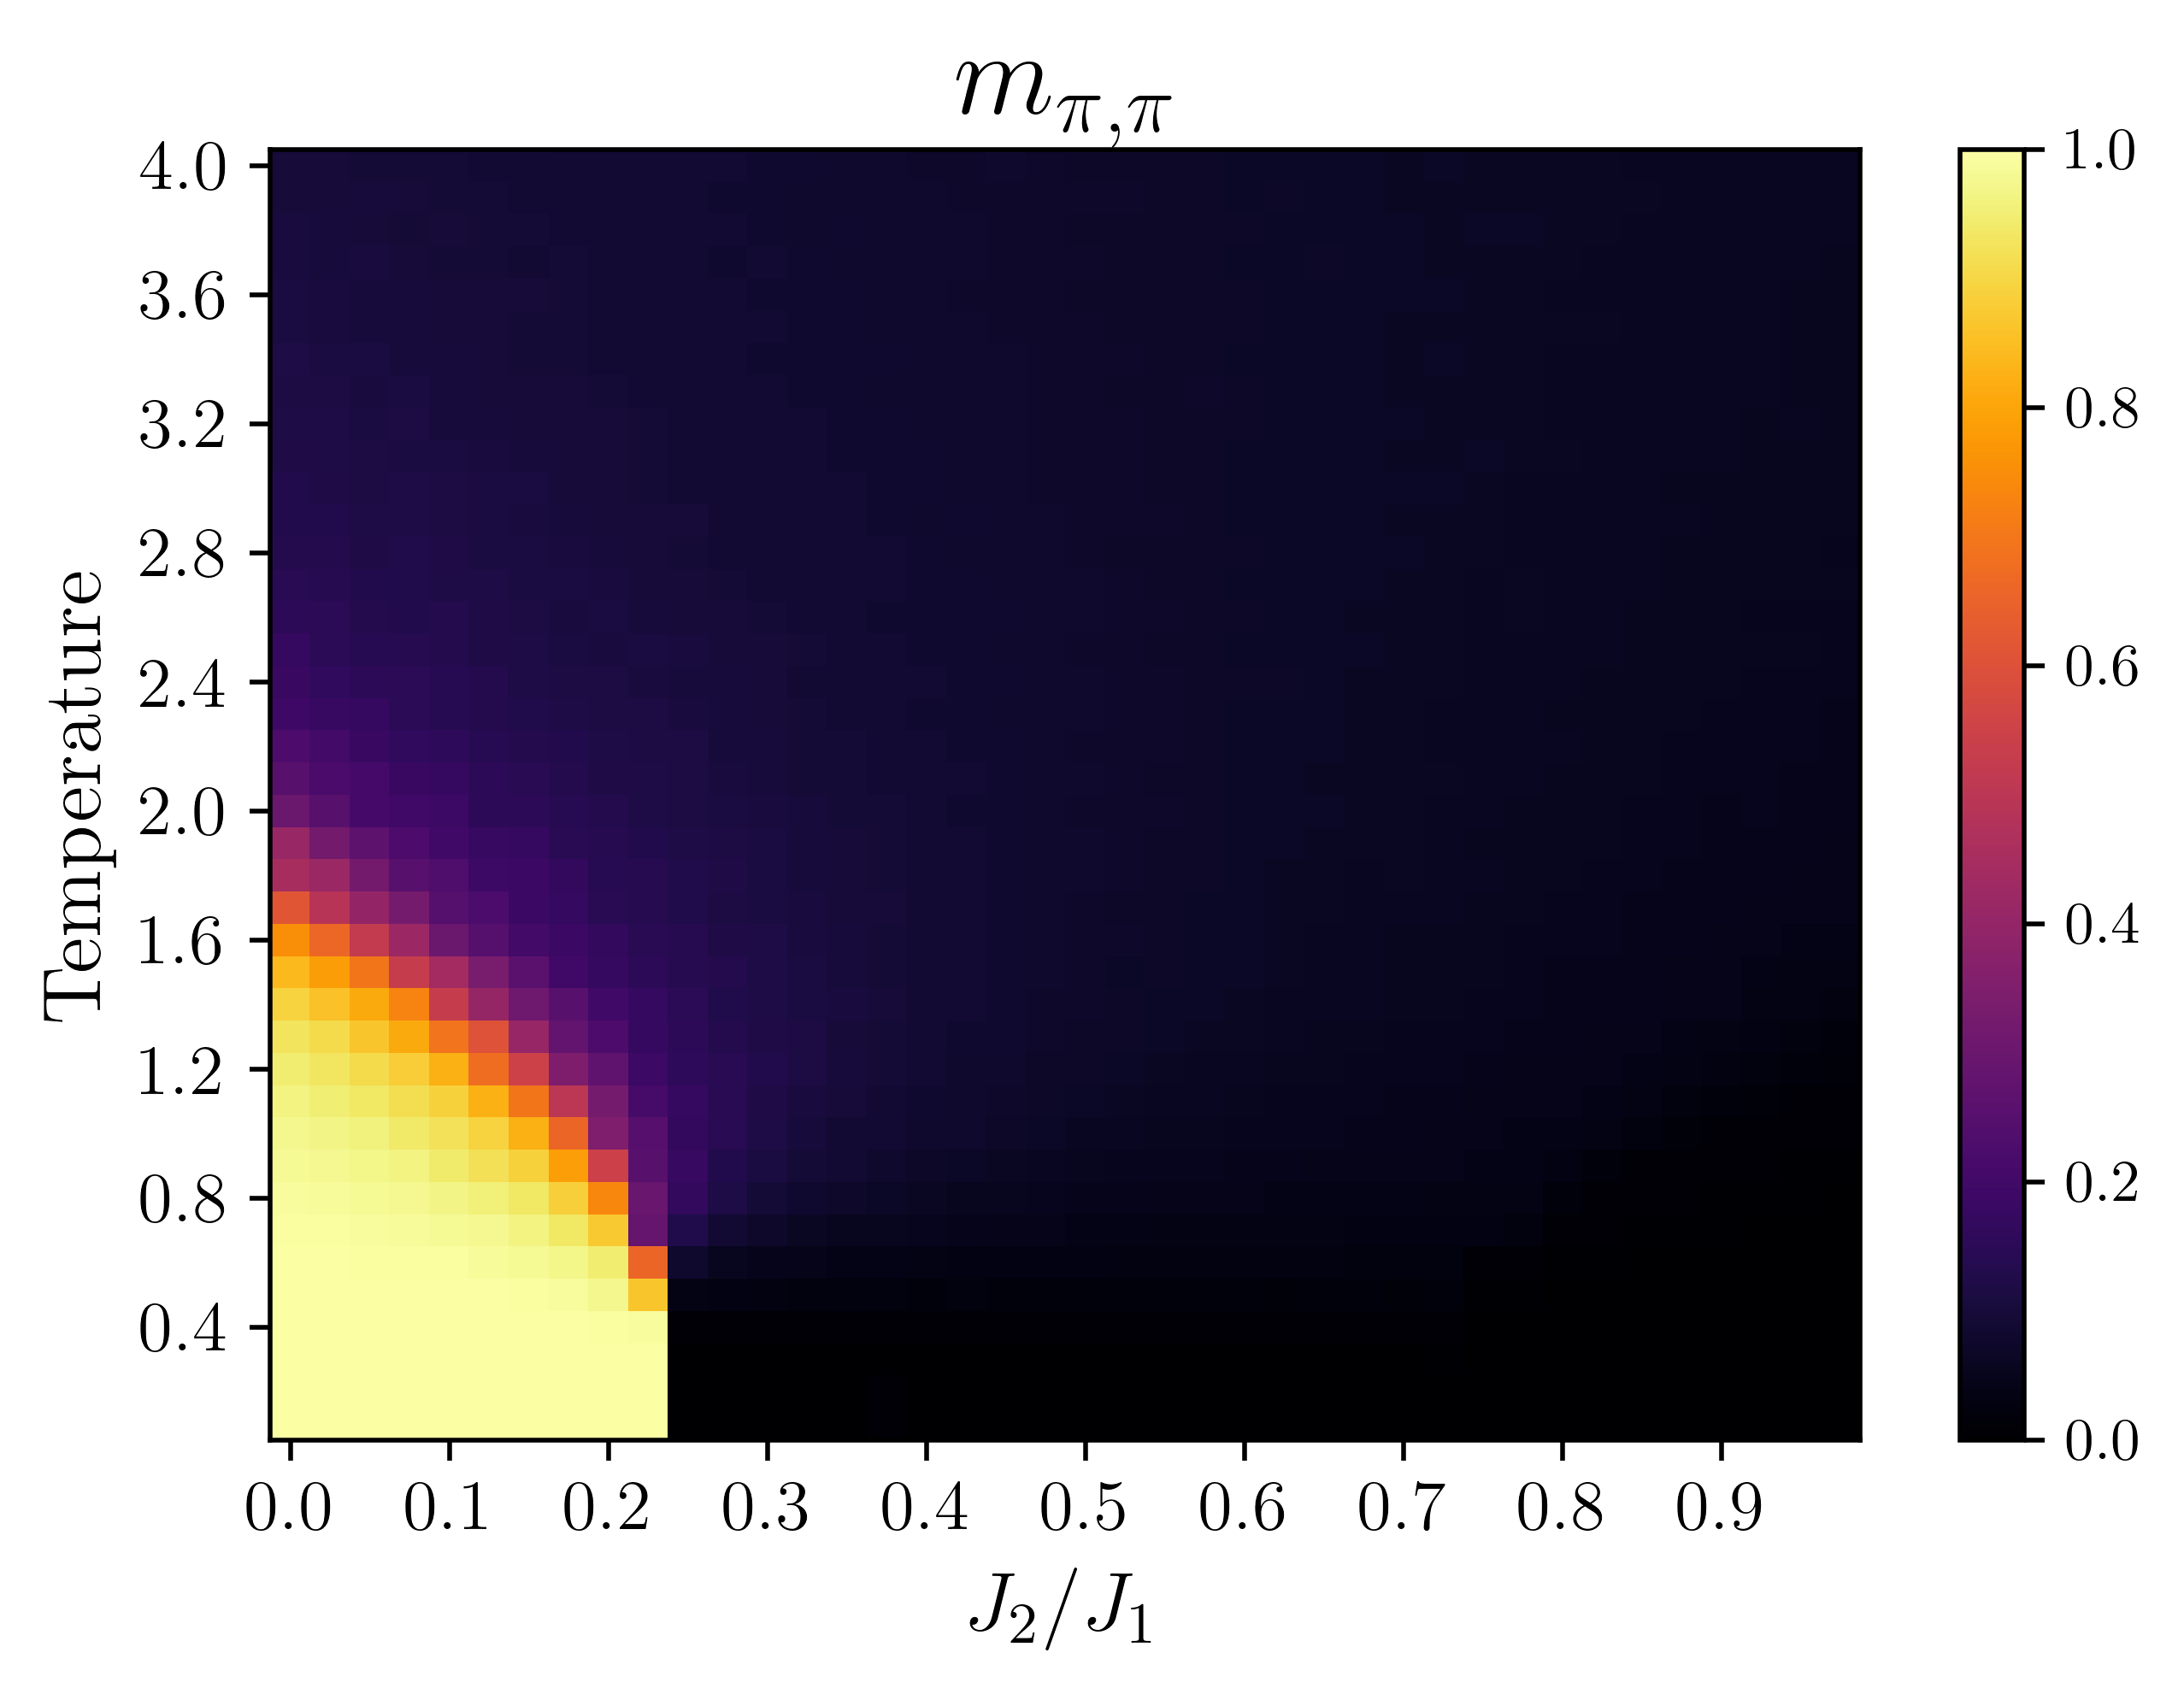
\includegraphics[width=\textwidth]{images/j1-j2/phase_diagrams/p=0.50/M_pi,pi_p=0.50.png}
    \end{subfigure}
    \begin{subfigure}[b]{0.43\textwidth}
        \centering
        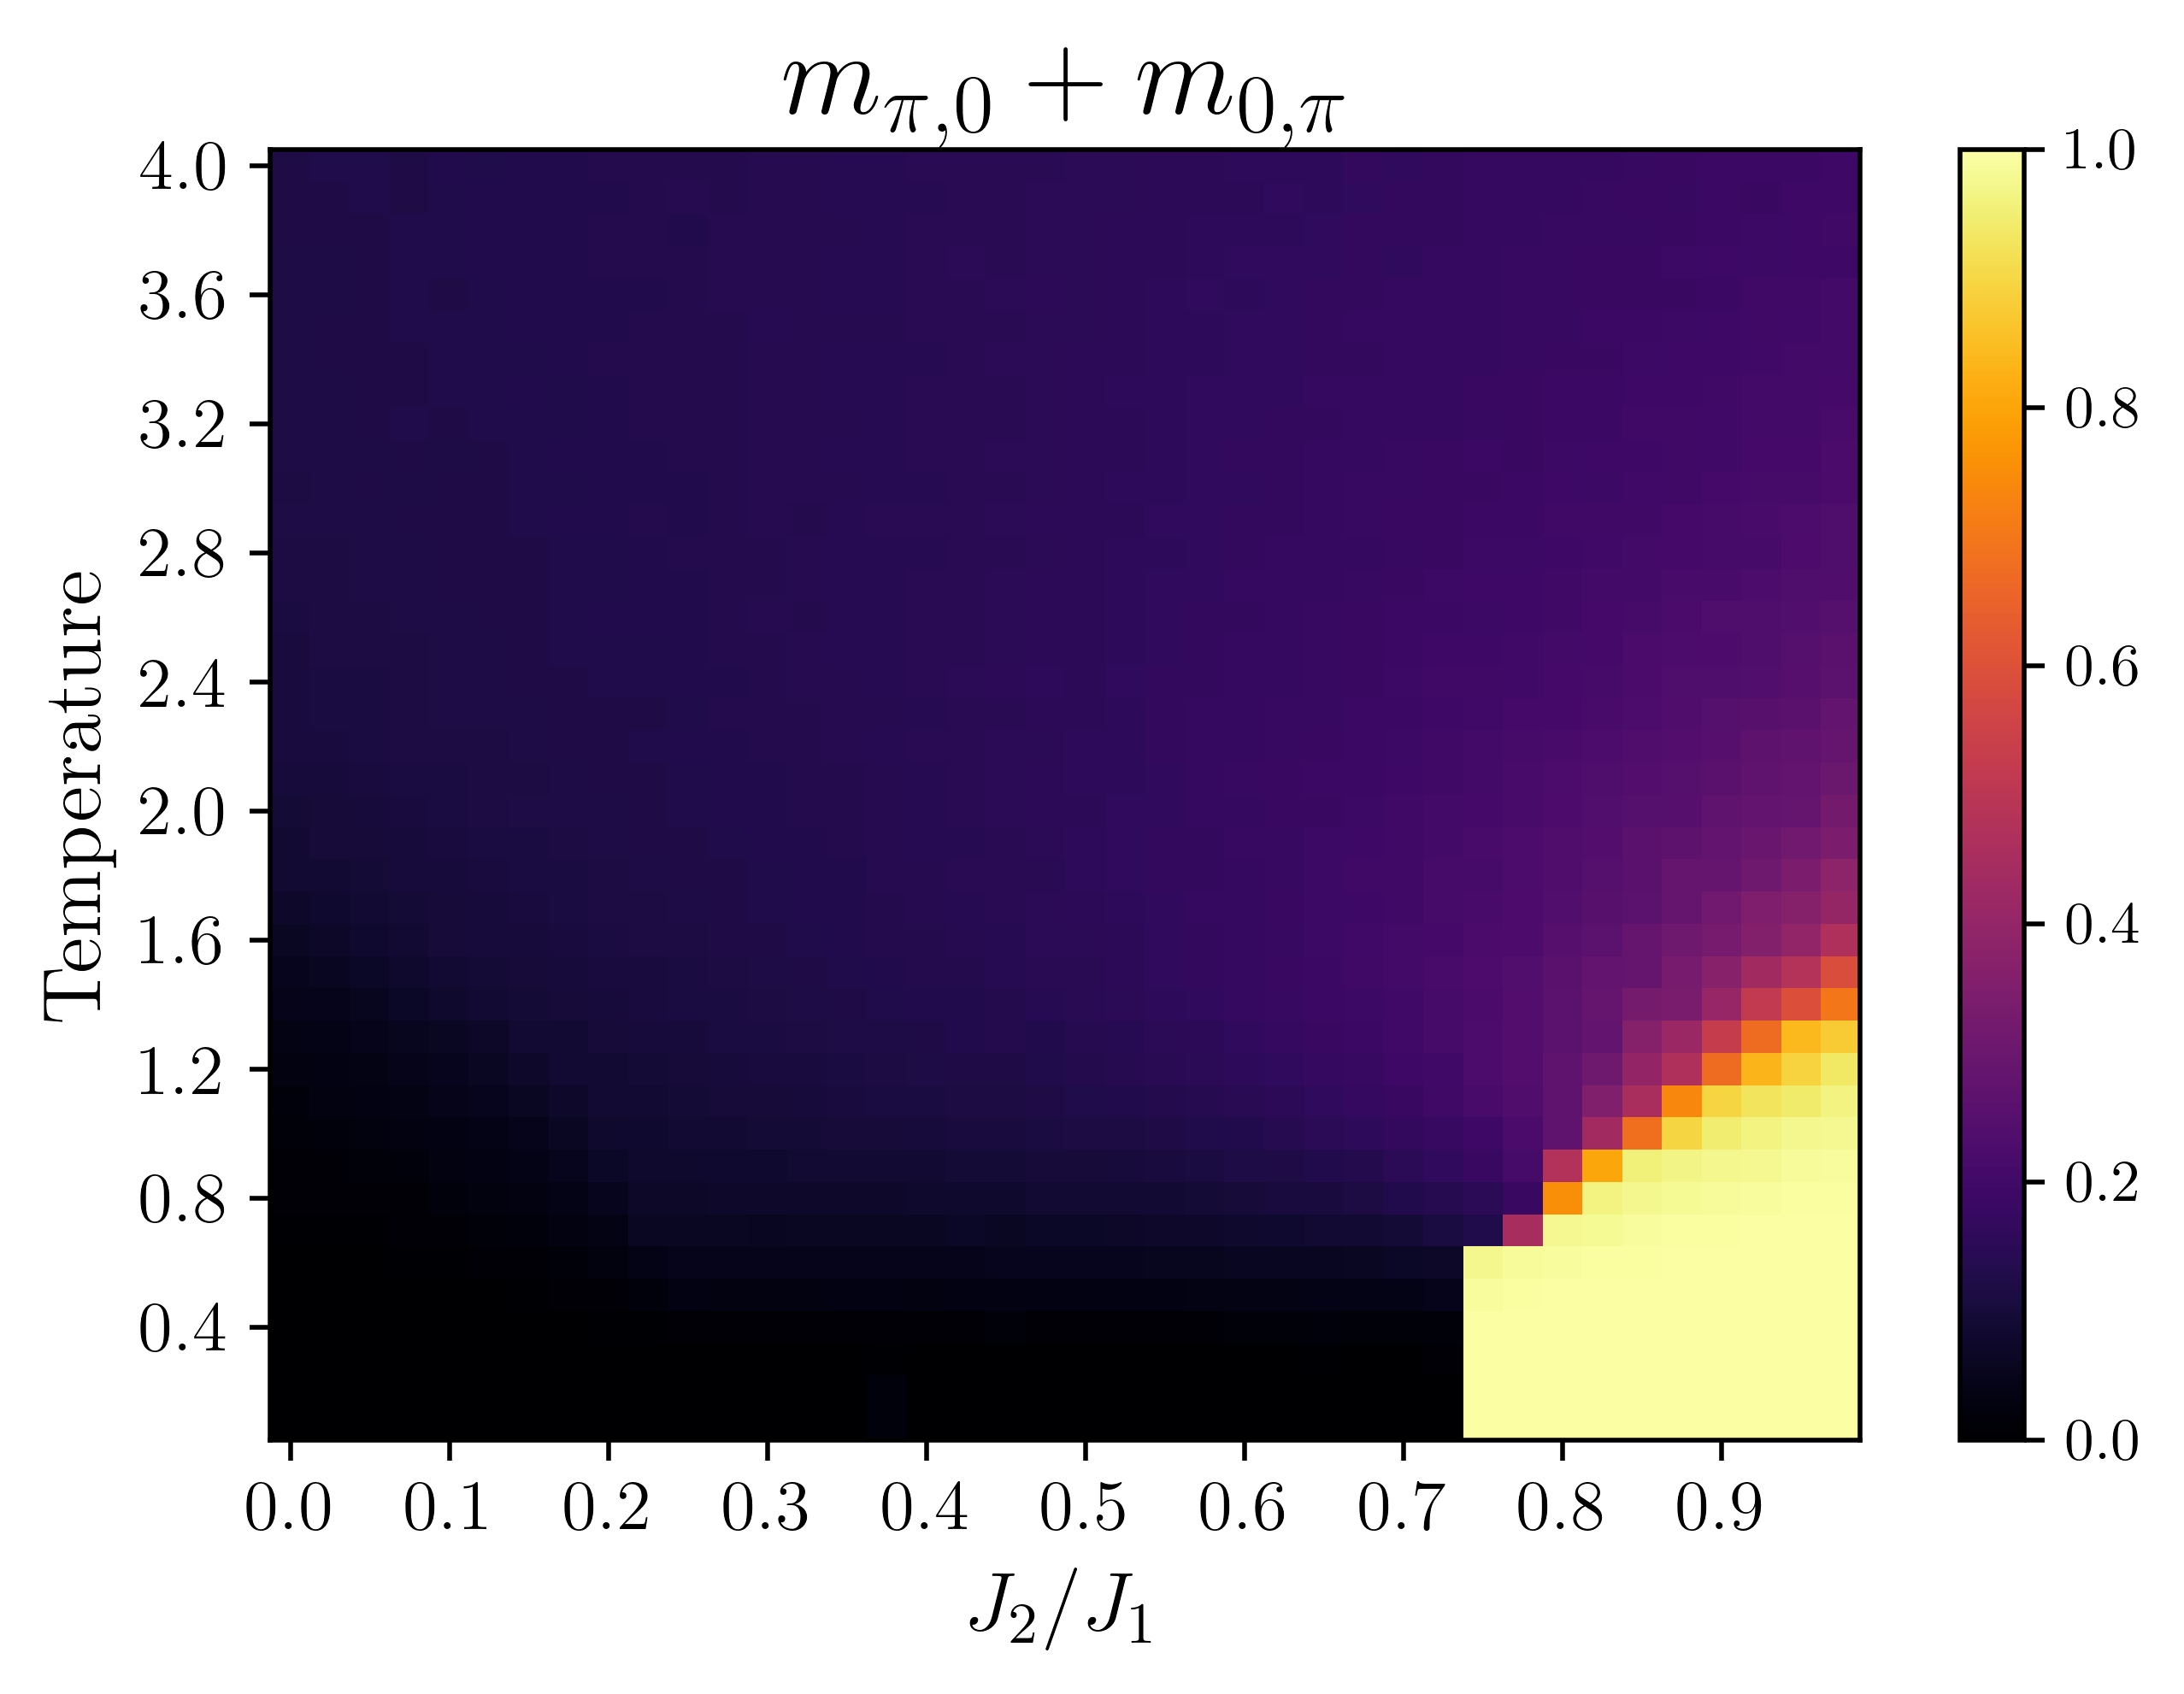
\includegraphics[width=\textwidth]{images/j1-j2/phase_diagrams/p=0.50/M_pi,0_p=0.50.png}
    \end{subfigure}
    \begin{subfigure}[b]{0.43\textwidth}
        \centering
        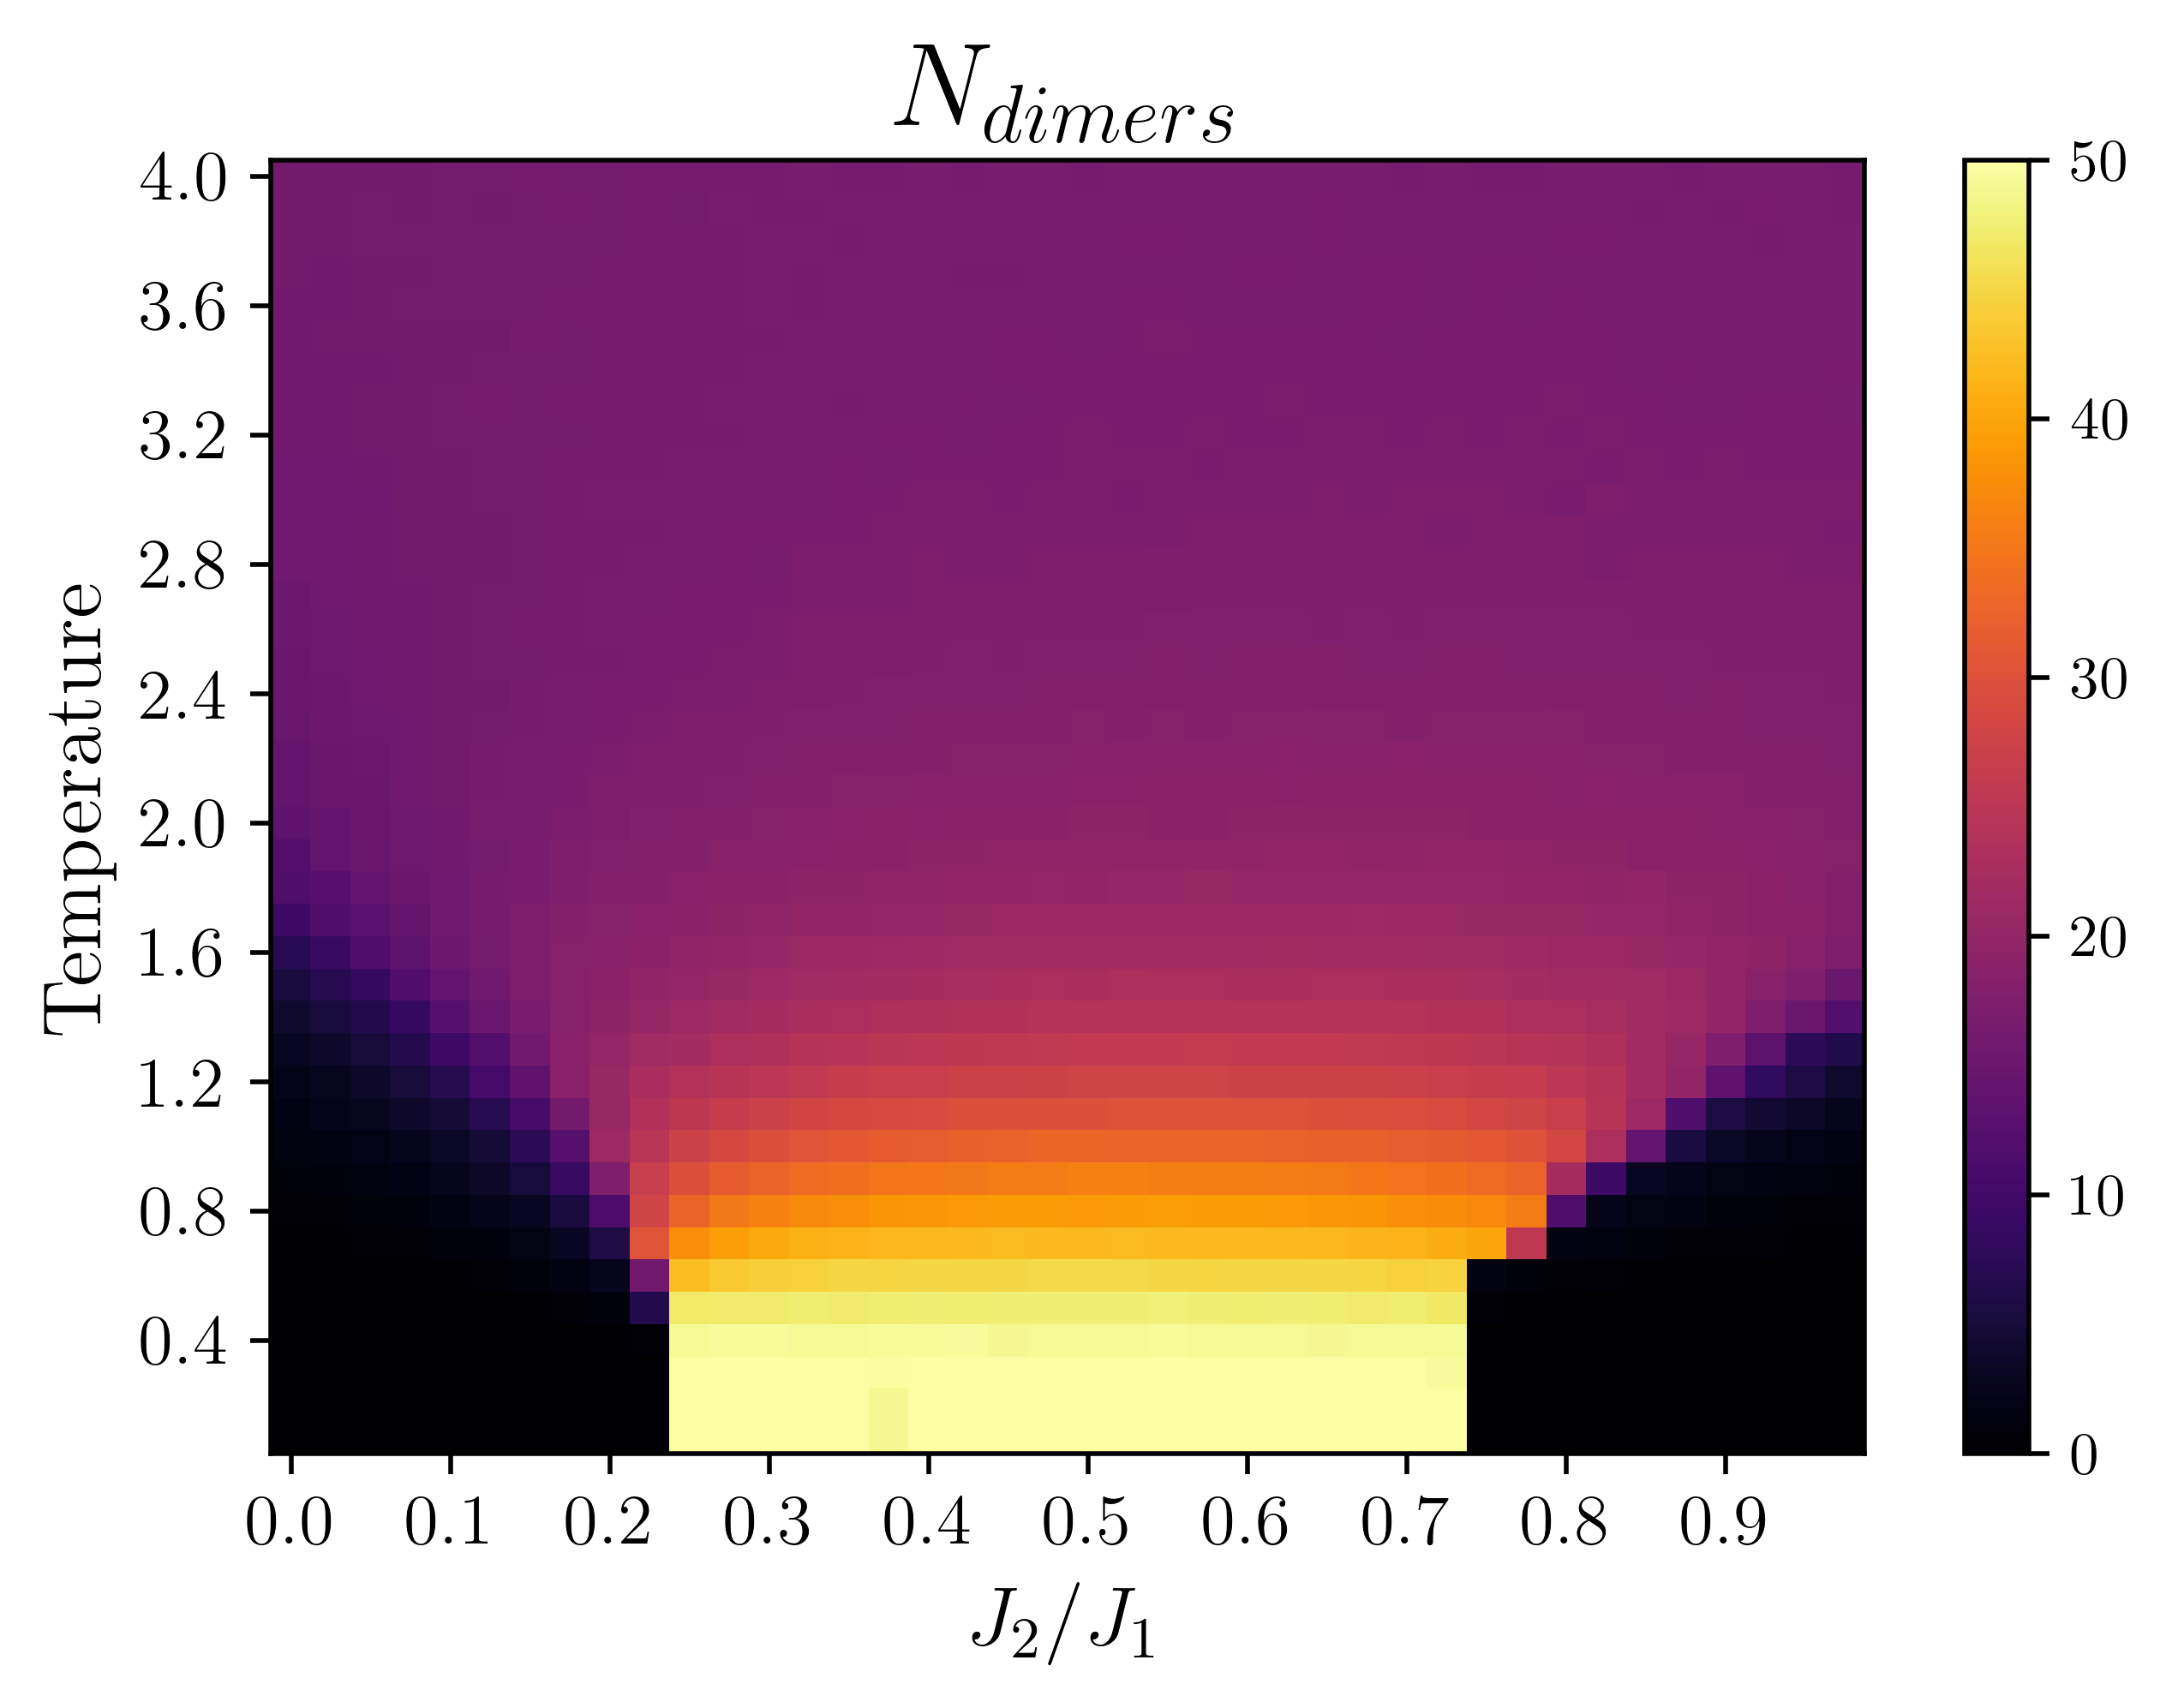
\includegraphics[width=\textwidth]{images/j1-j2/phase_diagrams/p=0.50/N_dimers_p=0.50.png}
    \end{subfigure}
    \caption{Order parameters at $p = 0.50$}
    \label{p=0.50}
\end{figure}
%%% FIG %%%
\FloatBarrier

\subsection{Entropic stabilization}
As discussed in Section \ref{t=0}, we saw that the quantum critical points ($T=0$) appear at $J_2/J_1 = 0.25$ and $J_2/J_1 = 0.75$ when argued from an energetic viewpoint. However, the spin liquid state is meta-stable only at extremely small temperatures and quickly destabilizes at temperatures of the order $\mathcal{O}(\texttt{1.0e-1})$. This is because the AFM state is entropically more favorable than a dimerized spin liquid state which has a much smaller set of configurations to explore. 
%%% FIG %%%
\begin{figure}[!htb]
    \centering
    \begin{subfigure}[b]{0.45\textwidth}  %keep total sum <1 to show in same line
        \centering
        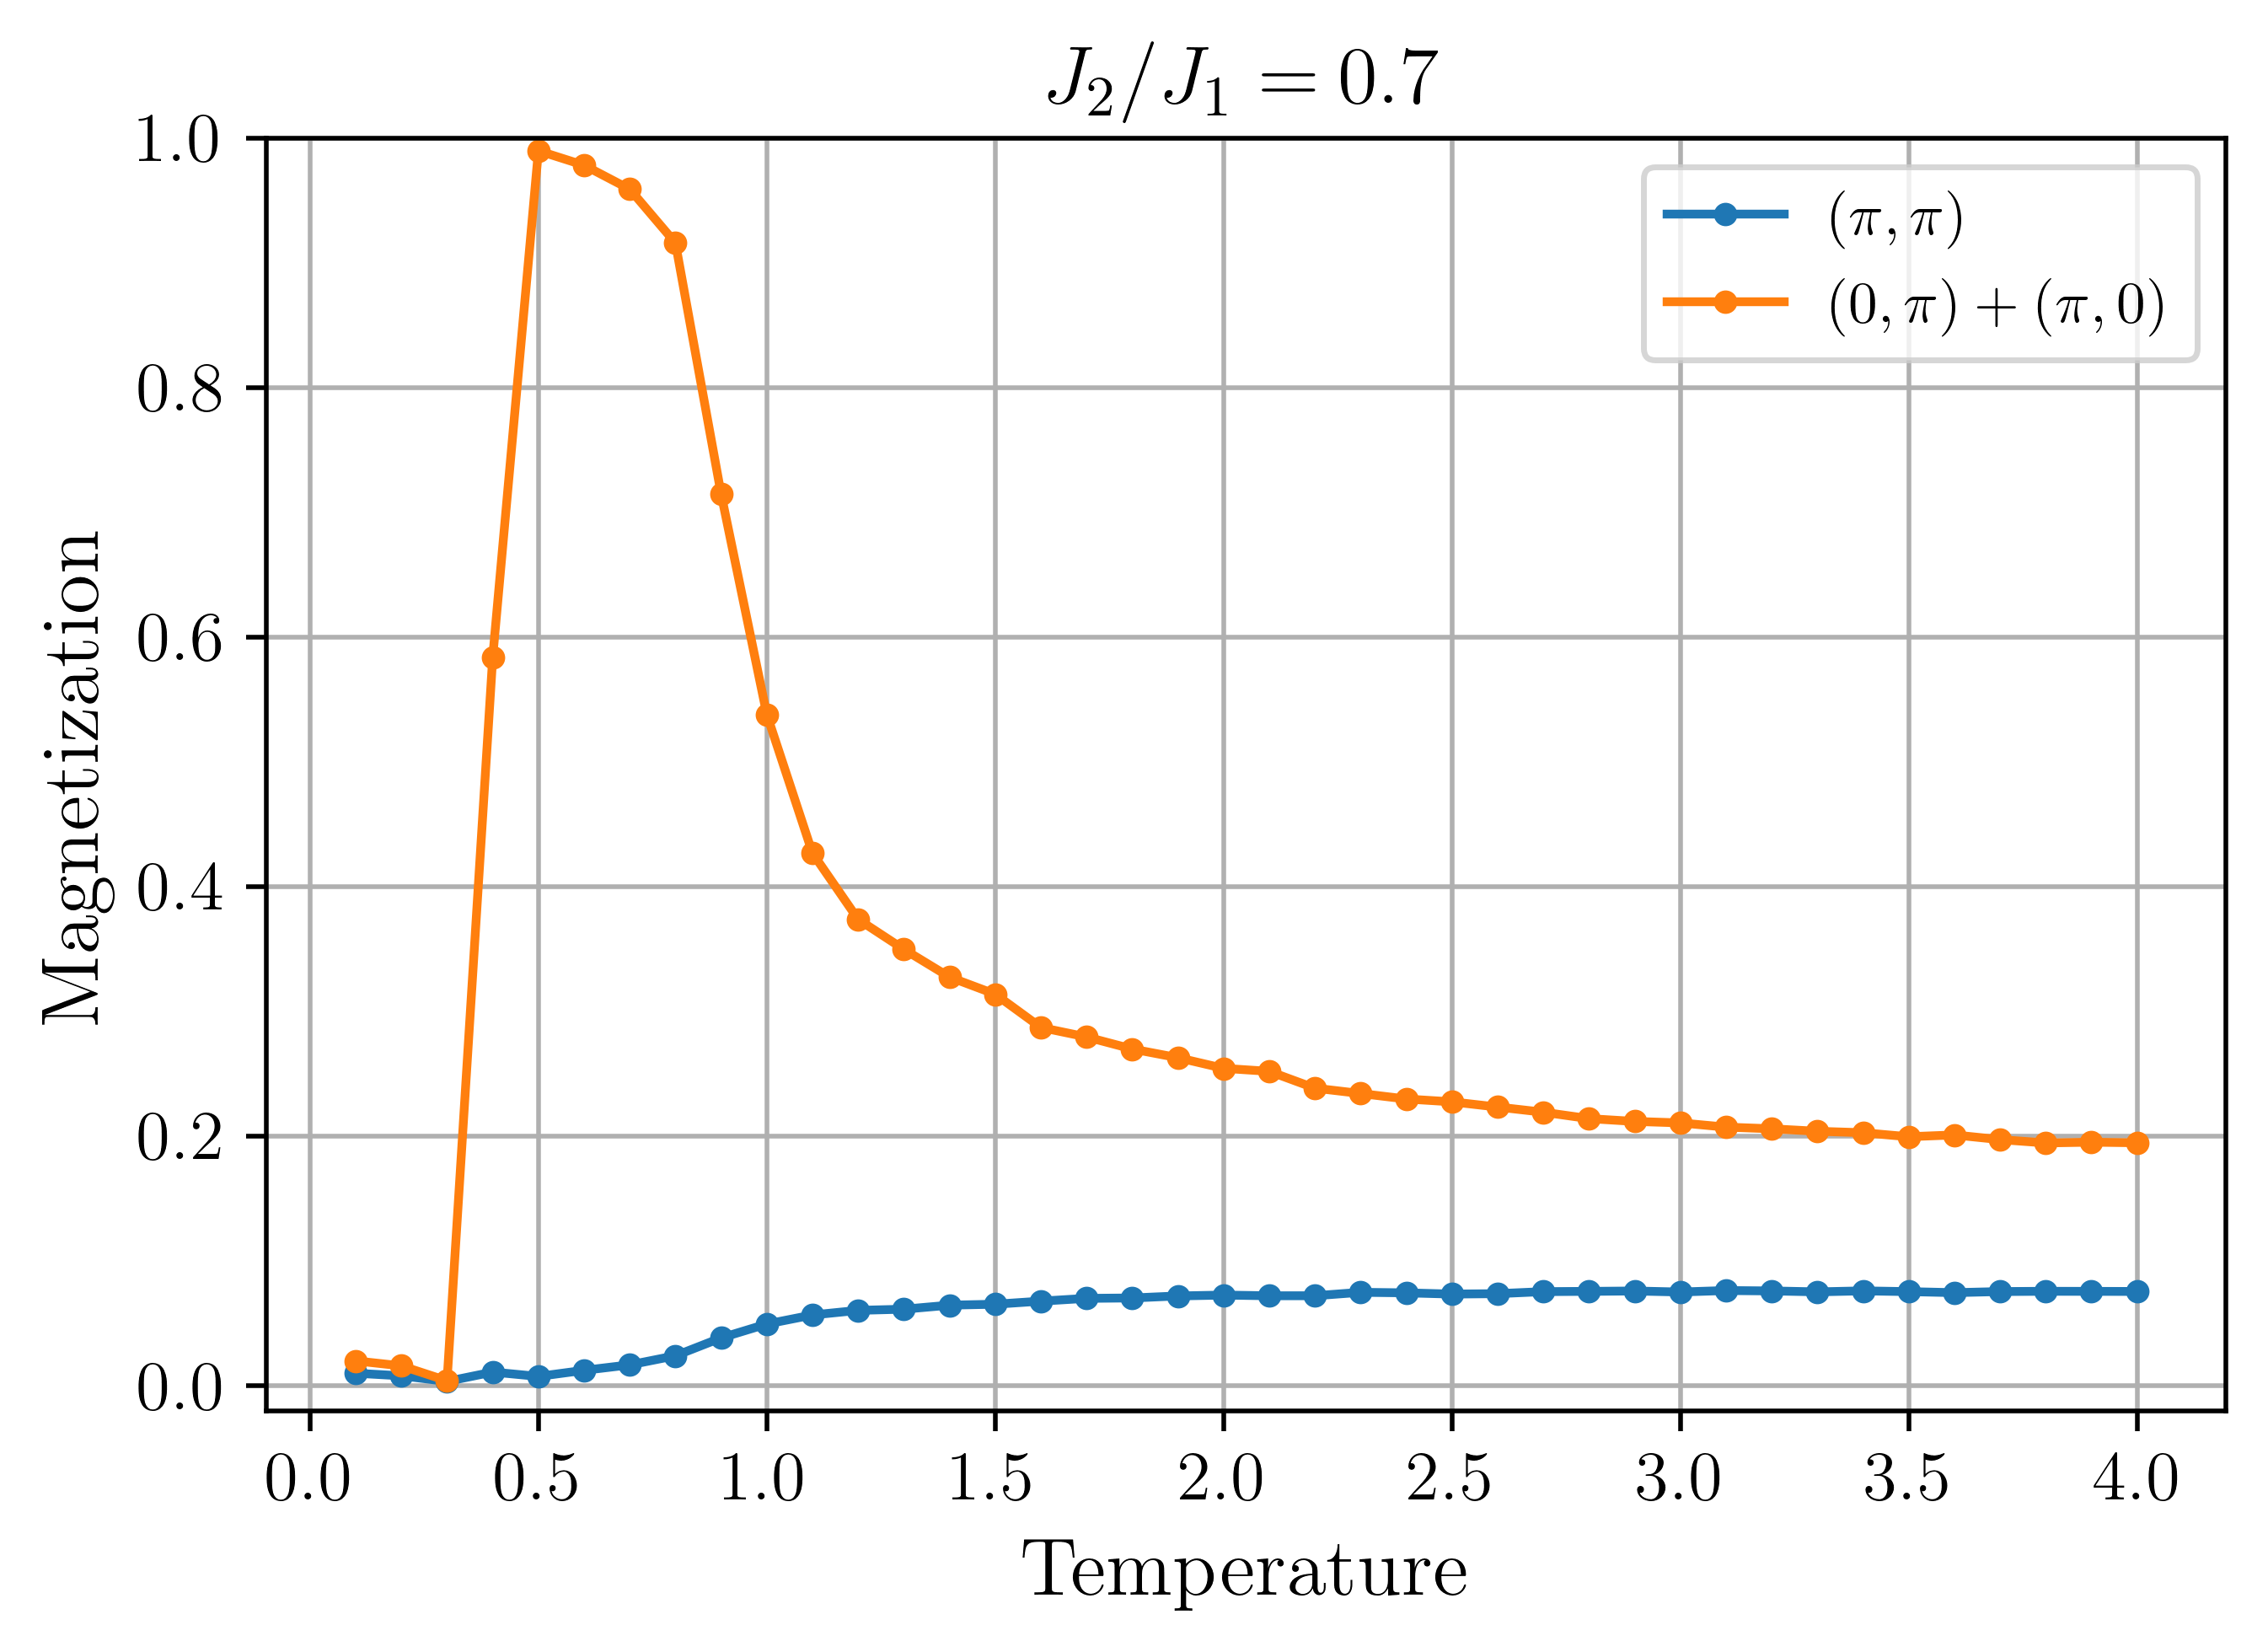
\includegraphics[width=\textwidth]{images/j1-j2/entropy_mag.png}
    \end{subfigure}
    \begin{subfigure}[b]{0.45\textwidth}
        \centering
        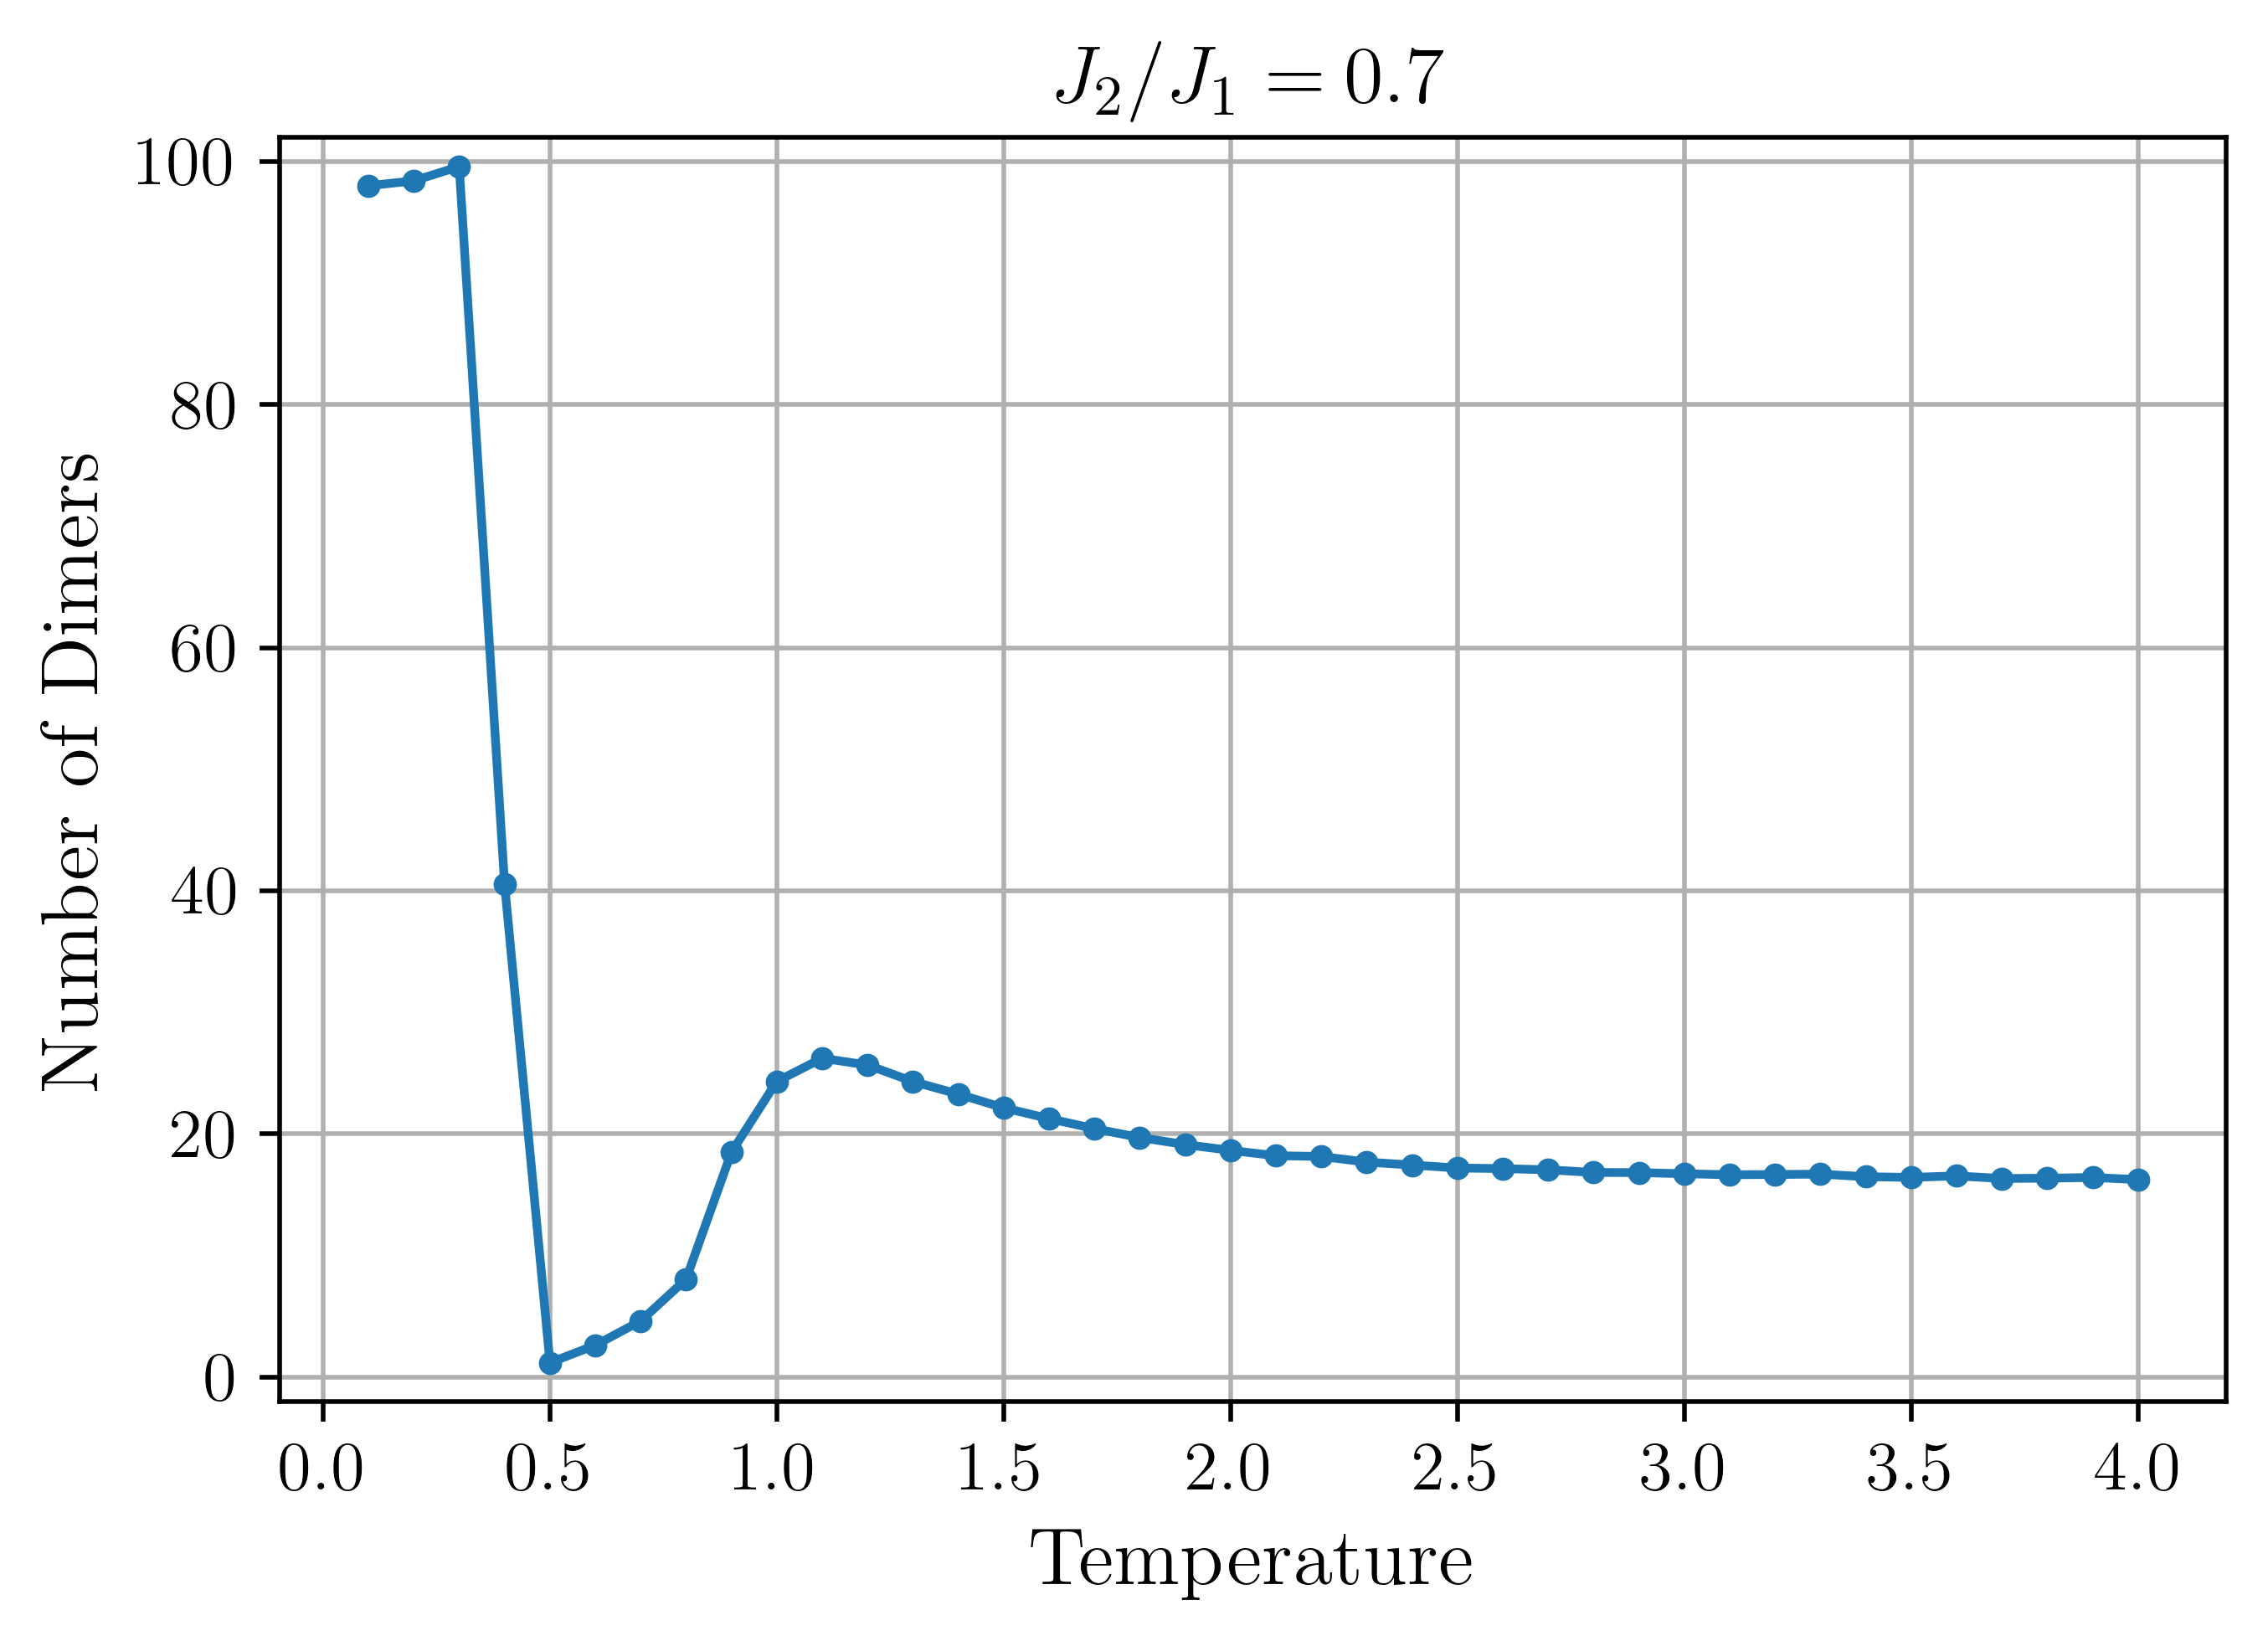
\includegraphics[width=\textwidth]{images/j1-j2/entropy_ndimer.png}
    \end{subfigure}
    \caption{Entropic stabilization of AFM and destabilization of the spin liquid state.}
    \label{}
\end{figure}
%%% FIG %%%
\FloatBarrier \!\!\!\!\!\!\!\!\!\!\!
This entropic stabilization process for the AFM state further pushes the boundaries of the phases and can be tuned via the parameter $p$ to give the correct phase transition points. It is, of course, necessary to provide a physical or a mathematical explanation for choosing the value of $p$ which gives the same results as a quantum Monte Carlo calculation.

\section{Summary and future outlook}
As demonstrated in this chapter, there is evidence that quantum spin models can be analyzed using a combination of  classical Monte Carlo simulations and singlet dimer dynamics, which accounts for the quantum fluctuations in the system. We see that the spin liquid phase emerges out of a semi-classical calculation, and is stable in roughly the correct region. The semi-classical simulations give the correct qualitative behavior, but we are still working on developing an accurate method which gives the correct phase boundaries of the resulting phases.

We also aim to work on evaluating whether the region between $0.4 \lessapprox {J_2}/{J_1} \lessapprox 0.6$ is actually a spin liquid phase or a valence bond state. This can be verified by calculating the singlet structure factor. We also aim to extend this approach to different spin models or different lattice geometries by defining a rigorous way to extract the quantum features of a model.
\end{document}